\documentclass[aspectratio=169]{beamer}

% Packages
\usepackage{amsthm}        % For theorems
\usepackage{amsmath}       % For math
\usepackage{luatexja}      % For Japanese
\usepackage{booktabs}      % For formal tables
\usepackage{mathtools}
\usepackage{amssymb}       % For checkmark
\usepackage{ulem}          % For strikeout
\usepackage[dvipsnames]{xcolor} % For colors (i.e. ForestGreen)
\usepackage[noend]{algpseudocode}
\usepackage[backend=biber,
            style=alphabetic,
            sorting=none
            ]{biblatex}    % For bibliography
\usepackage{tikz}          % For figures
\usepackage{multirow}      % For multirow in tables
\usetikzlibrary{arrows.meta,
                chains,
                positioning}
\addbibresource{references.bib}

% Custom commands
\DeclareMathOperator{\interior}{int}
\DeclareMathOperator{\sgn}{sgn}

% Beamer settings
\setbeamertemplate{theorems}[numbered]
\addtobeamertemplate{theorem begin}{\normalfont}{}
\newtheorem*{theorem*}{Theorem (restated)}
\newtheorem*{lemma*}{Lemma (restated)}
\newtheorem*{sproof}{Sketch of the proof.}
\newtheorem{remark}[theorem]{Remark}
\newtheorem{observation}[theorem]{Observation}

\newcommand{\info}[1]{\textcolor{ForestGreen}{#1}}

% Theme
\usetheme{metropolis}
\usecolortheme{default}
\metroset{block=fill}

% Fonts
\setbeamerfont{title}{size=\large,series=\bfseries}
\setbeamerfont{theorem}{shape=\upshape}
\usefonttheme{professionalfonts}
\usefonttheme{structurebold}
\setbeamerfont{title}{size=\LARGE}
\setbeamerfont{date}{size=\small}
\setbeamerfont{frametitle}{size=\large,series=\bfseries}
\setmainfont{Latin Modern Roman}
\usepackage{luatexja-fontspec}
\usepackage[T1]{fontenc}
\usepackage{mlmodern}
\usepackage{luatexja-otf}
\renewcommand{\kanjifamilydefault}{\gtdefault} % 既定欧文フォントがサンセリフなので，既定和文フォントもゴシック体に設定する
\renewcommand{\familydefault}{\sfdefault}

% Metadata
\title{5.4 最適化問題の整数計画問題による定式化}
\subtitle{近似アルゴリズム ―離散最適化問題への効果的アプローチ―}
\author{岡山 大輝}
\institute{兵庫県立大学大学院 情報科学研究科\textit{(ad25r010@guh.u-hyogo.ac.jp)}}
\date{August 26, 2025}

\begin{document}

\begin{frame}
	\titlepage
\end{frame}

\begin{frame}{はじめに}
	\vskip 2em
	\begin{quote}
		In order to appreciate the role of \alert{LP-duality theory} in approximation algorithms, it is important to first understand its role in \alert{exact algorithms}.
		\vskip5mm
		\hspace*\fill{\small--- Vijay Virkumar Vazirani}
	\end{quote}
	\begin{figure}
		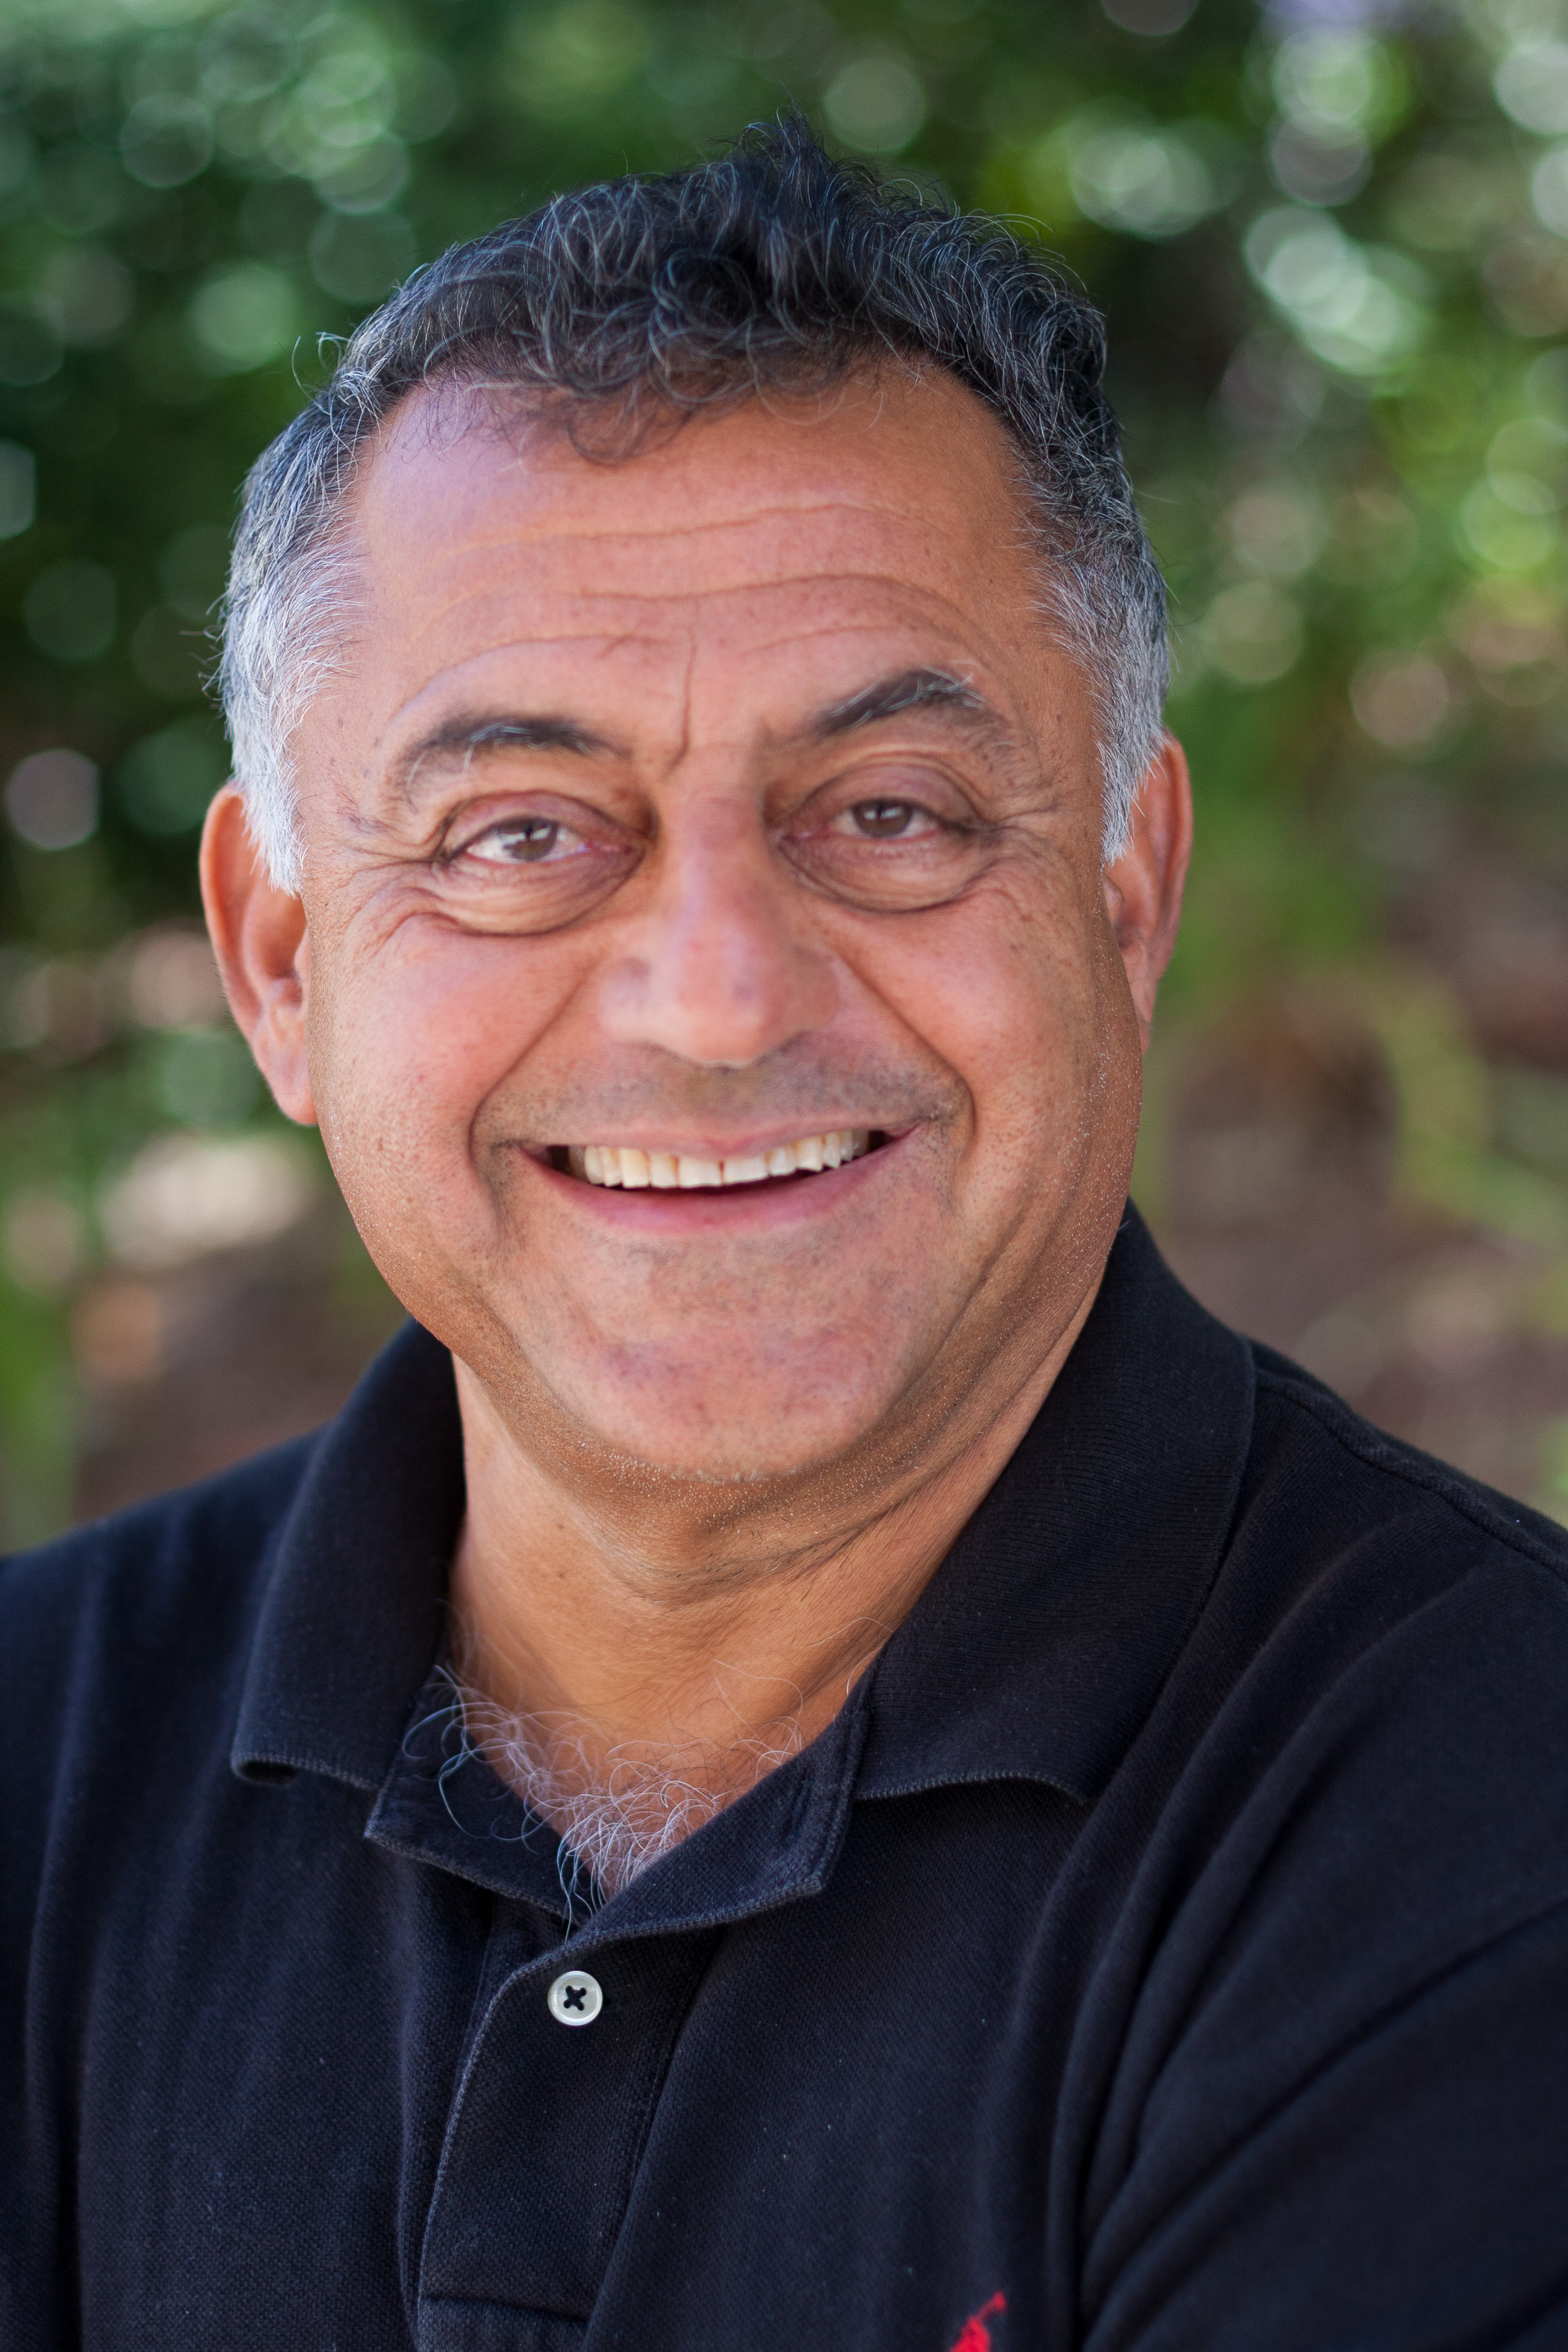
\includegraphics[width=0.15\textwidth]{figures/vazirani.jpg}
		\caption{Vijay Virkumar Vazirani (1957-)}
	\end{figure}
\end{frame}

\begin{frame}{本発表のテーマ}
	\begin{theorem}[最大フロー最小カット定理]
		任意の有向グラフにおいて，始点と終点が与えられたとき，\alert{最大フロー}の値は\alert{最小カット}の容量に等しい．
	\end{theorem}

	% \begin{itemize}
	% 	\item 最大フロー問題を線形最適化問題として定式化する
	% 	\item その双対問題が最小カット問題の整数最適化問題の LP-緩和であることを示す
	% 	\item 双対問題が常に整数最適解をもつことを示す
	% 	\item LP-双対定理を利用して，最大フローと最小カットの値が等しいことを示す
	% \end{itemize}

	\begin{figure}
		\centering
		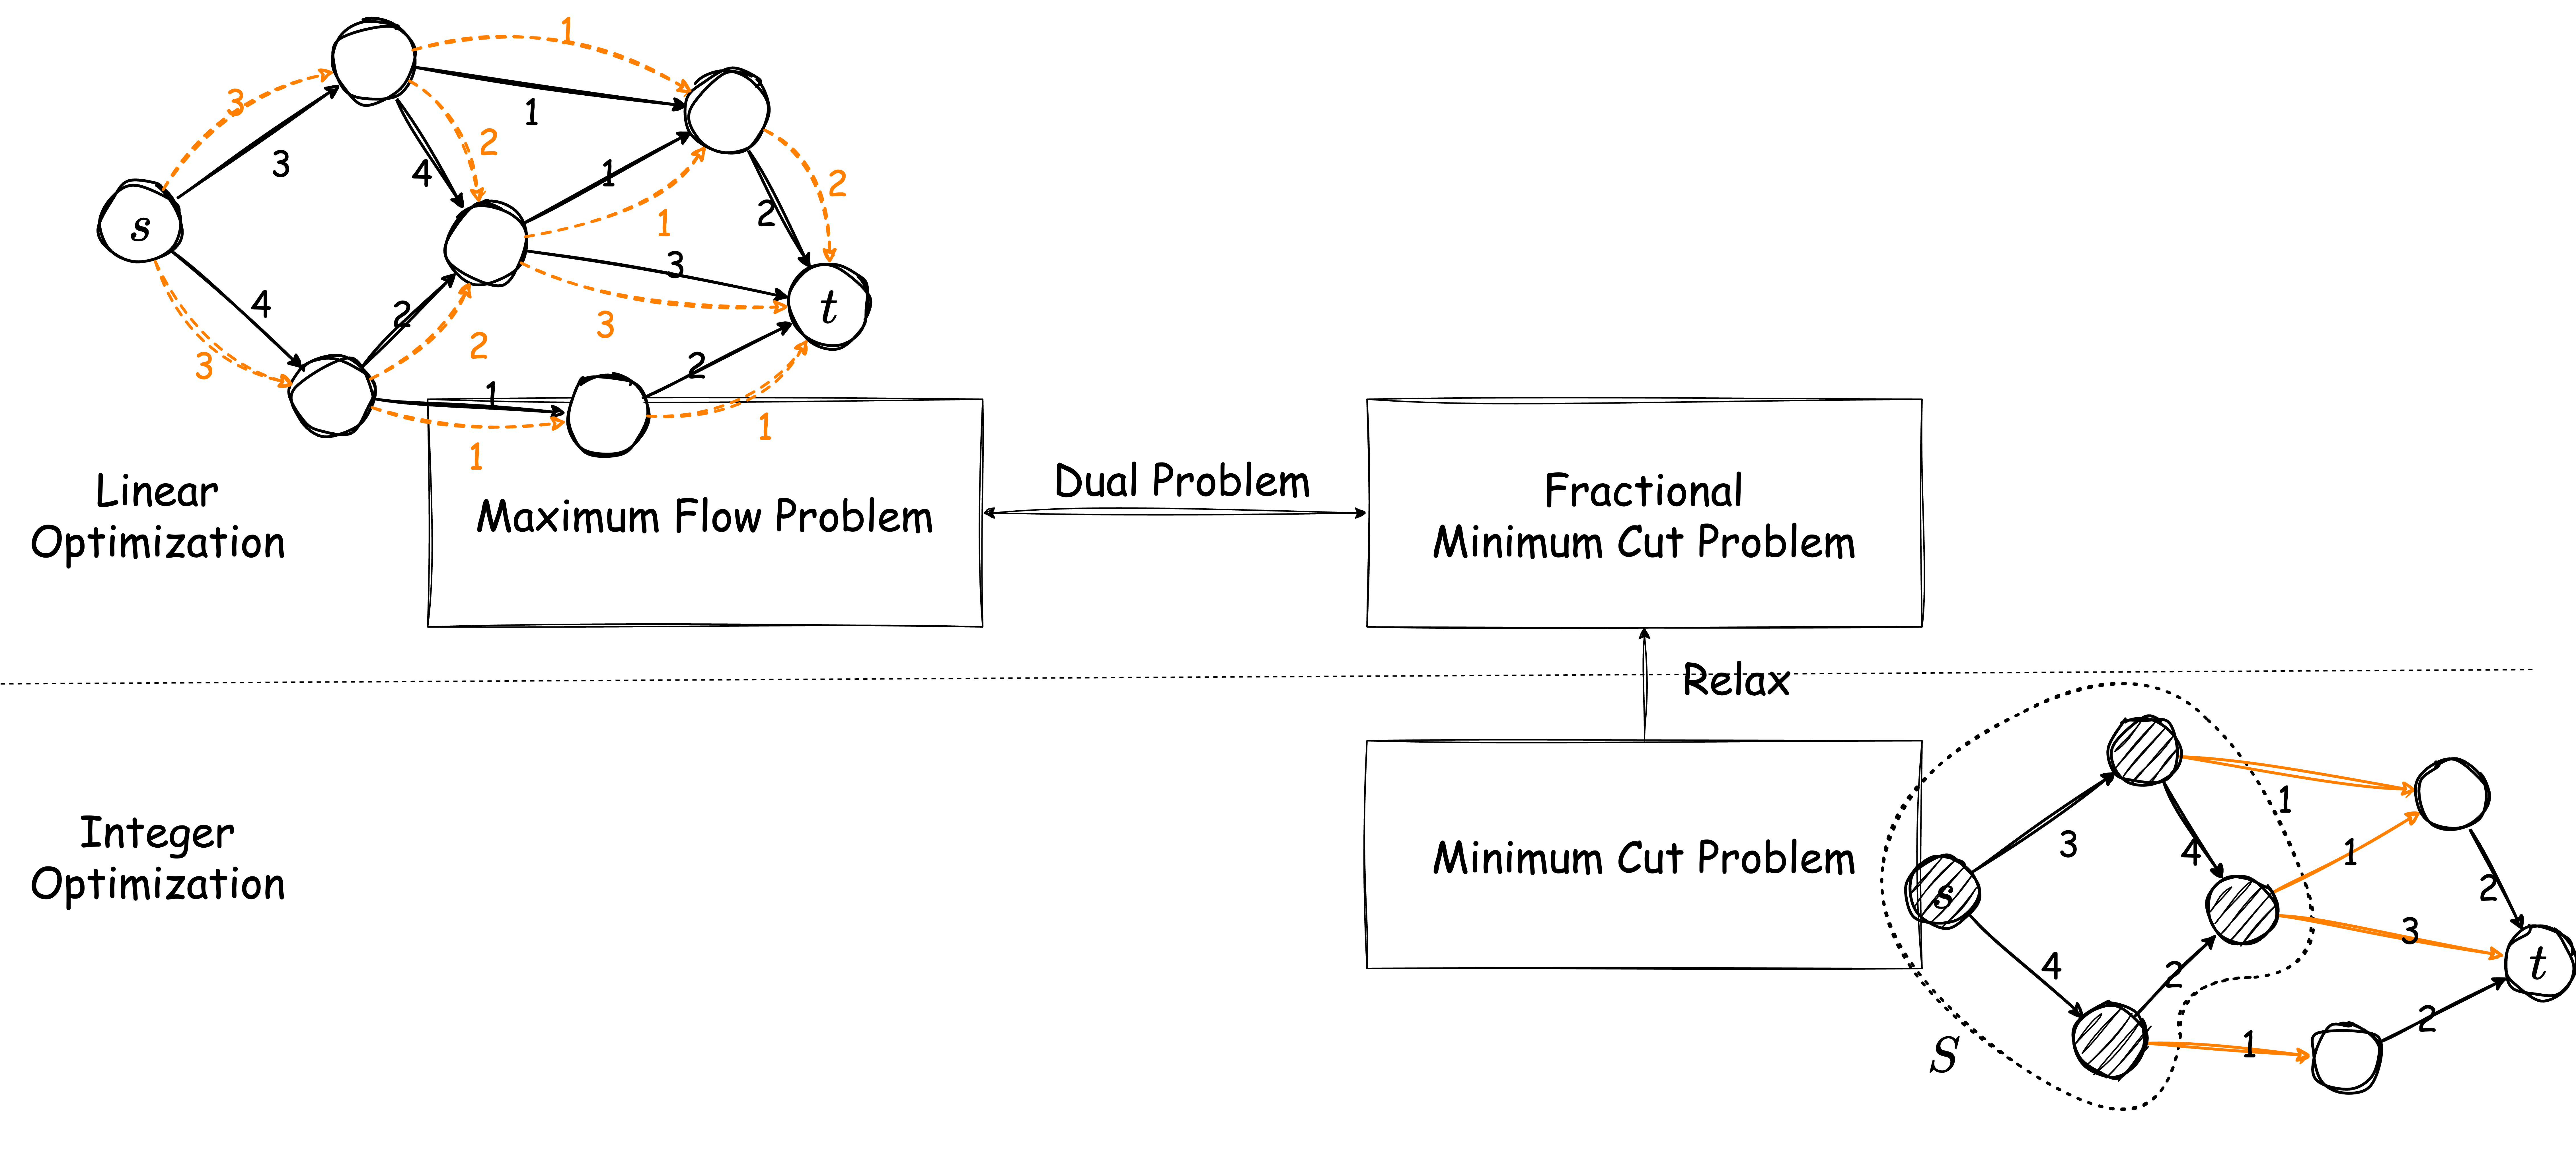
\includegraphics[width=0.9\textwidth]{figures/overview.drawio.png}
	\end{figure}

	\note{
		\begin{enumerate}
			\item 最大フロー問題を線形最適化問題として定式化する
			\item その双対問題の変数の制約を強めた問題が最小カット問題と等価であることを示す
		\end{enumerate}
	}
\end{frame}

\begin{frame}{フローとカット}
	有向グラフ \(G = (V, E)\) と各辺の容量 \(c: E \to \mathbb{R}_{+}\) が与えられる．
	\begin{columns}
		\begin{column}{0.46\textwidth}
			\begin{definition}[フロー]
				フローとは，容量制約と流入流出制約を満たす関数 \alert{\(f : E \to \mathbb{R}_{\ge 0}\)} である．
			\end{definition}

			\begin{figure}
				\centering
				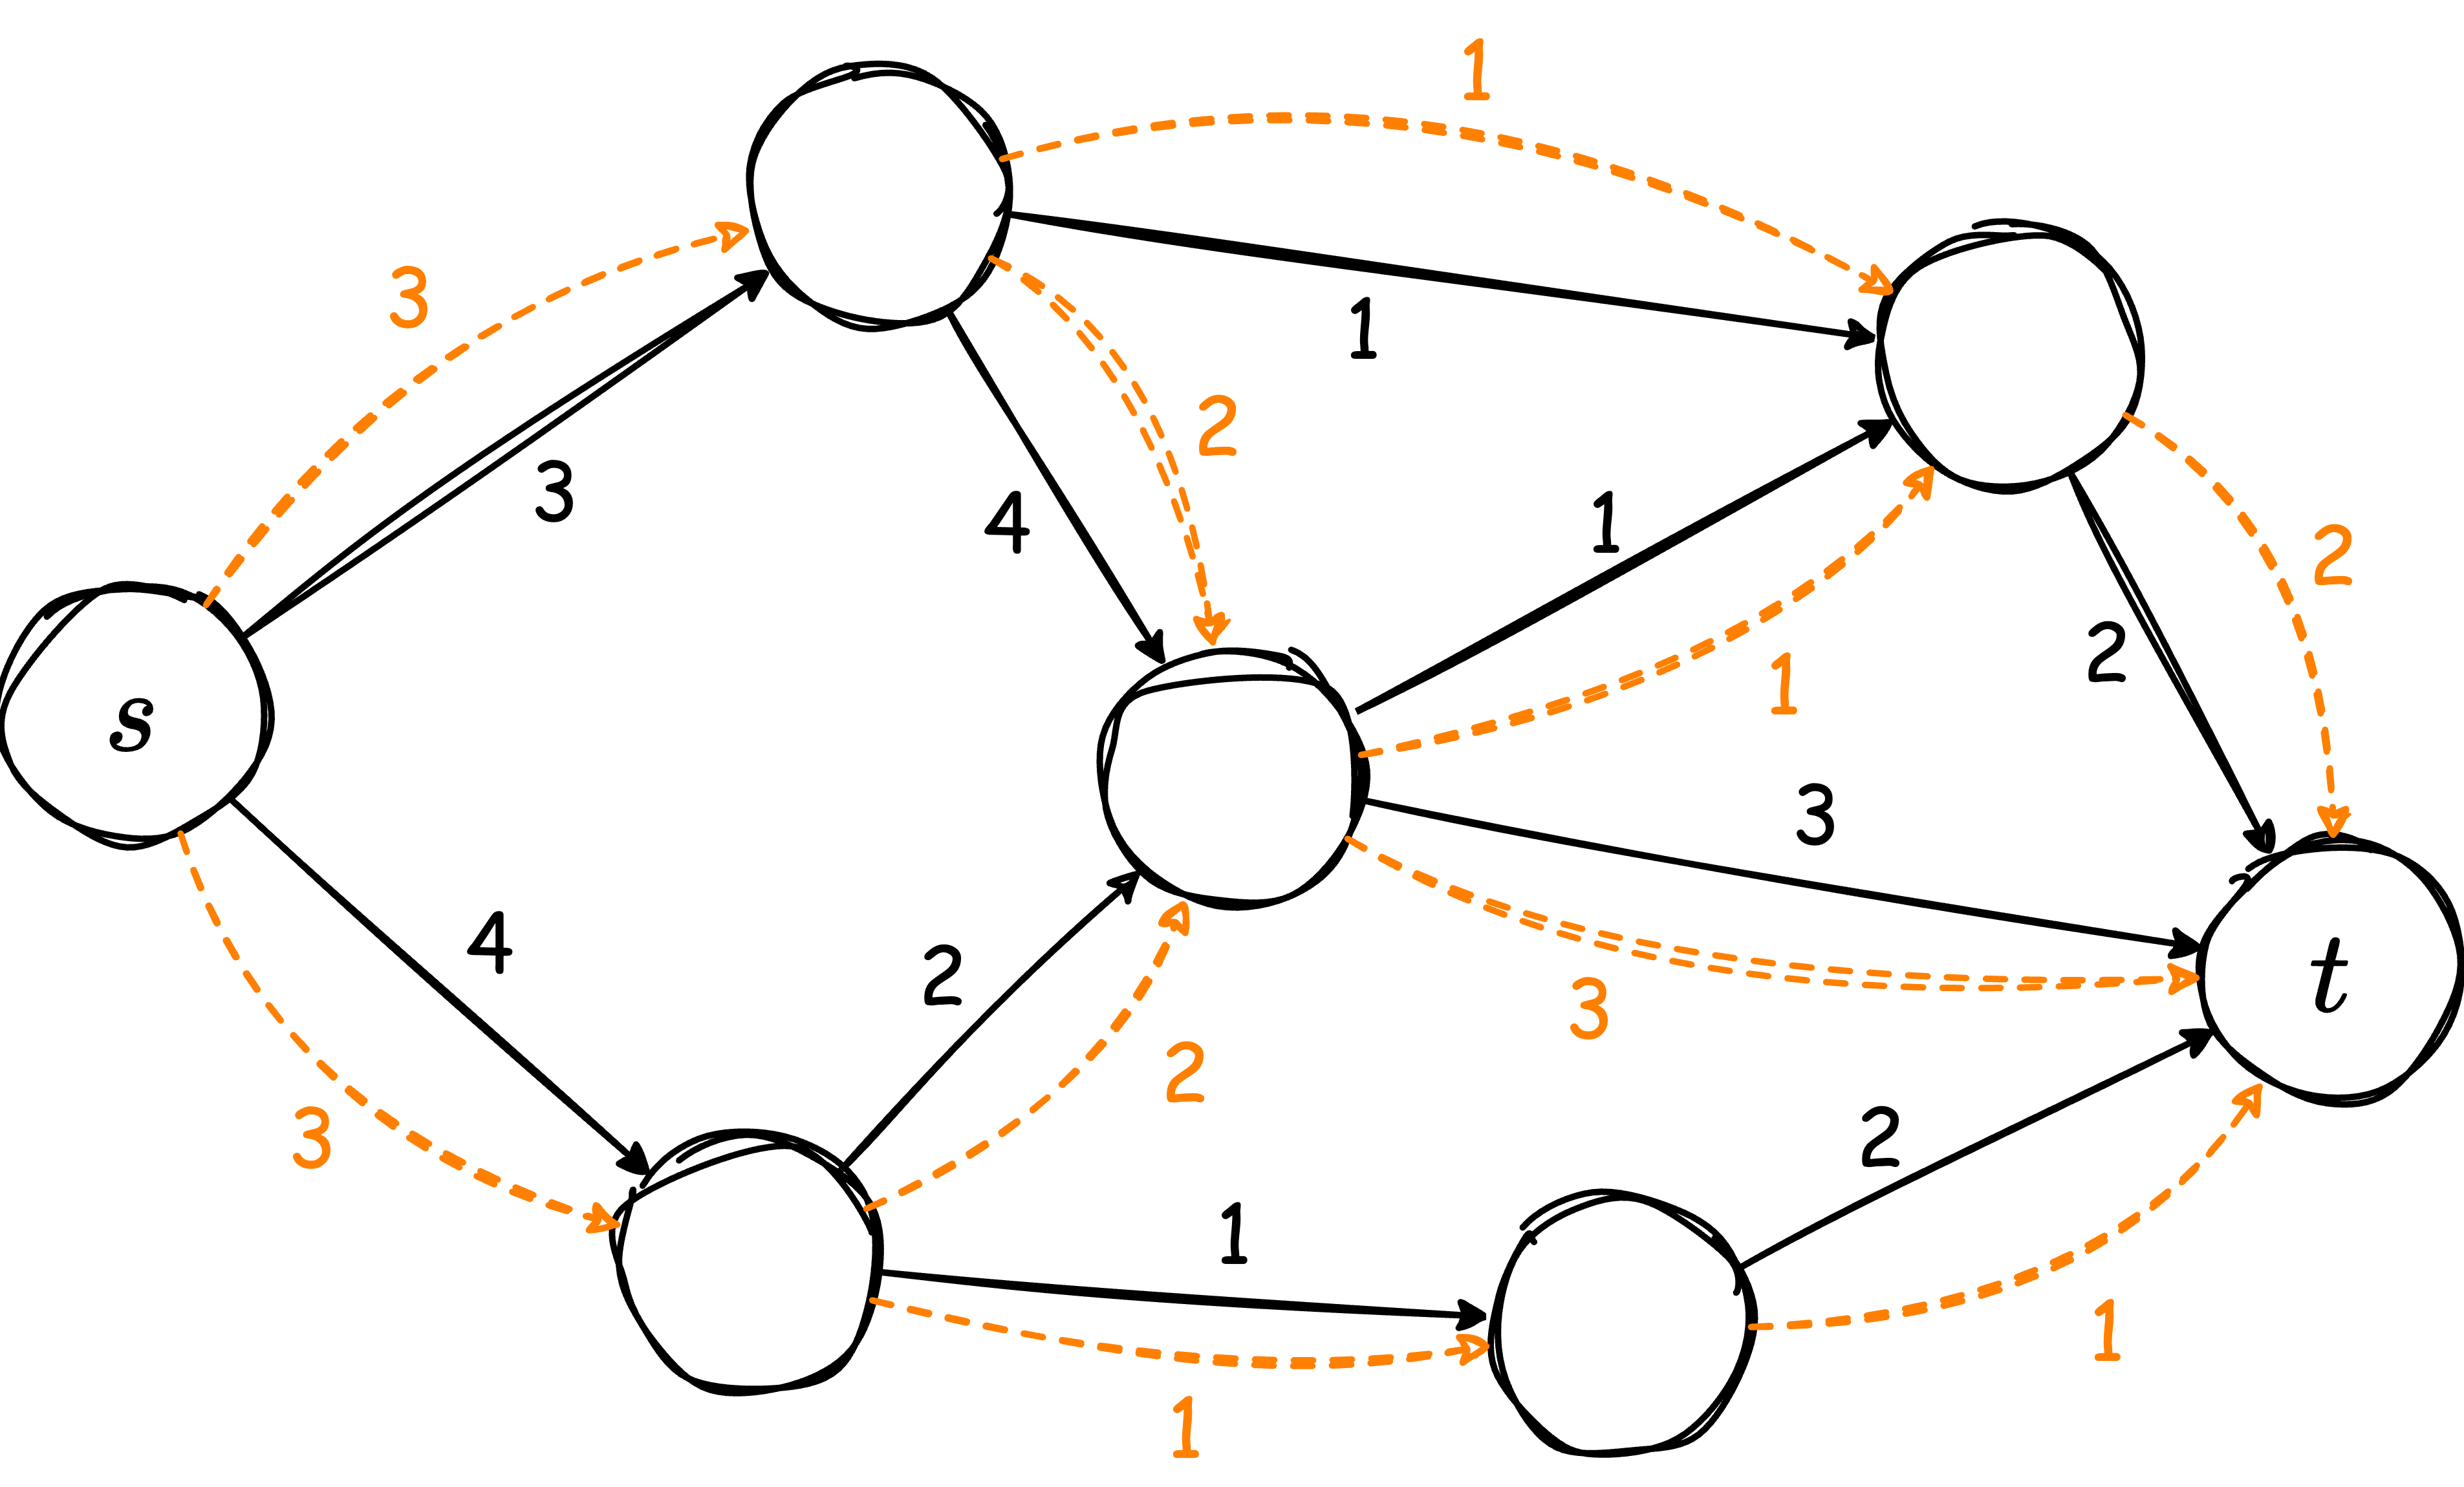
\includegraphics[width=1.0\textwidth]{figures/flow-example.drawio.png}
			\end{figure}

		\end{column}
		\begin{column}{0.46\textwidth}
			\begin{definition}[カット]
				カットとは，頂点集合 \(S \subseteq V\) により定義される \alert{\(S\) から \(V \setminus S\) への辺の集合}である．
			\end{definition}

			\begin{figure}
				\centering
				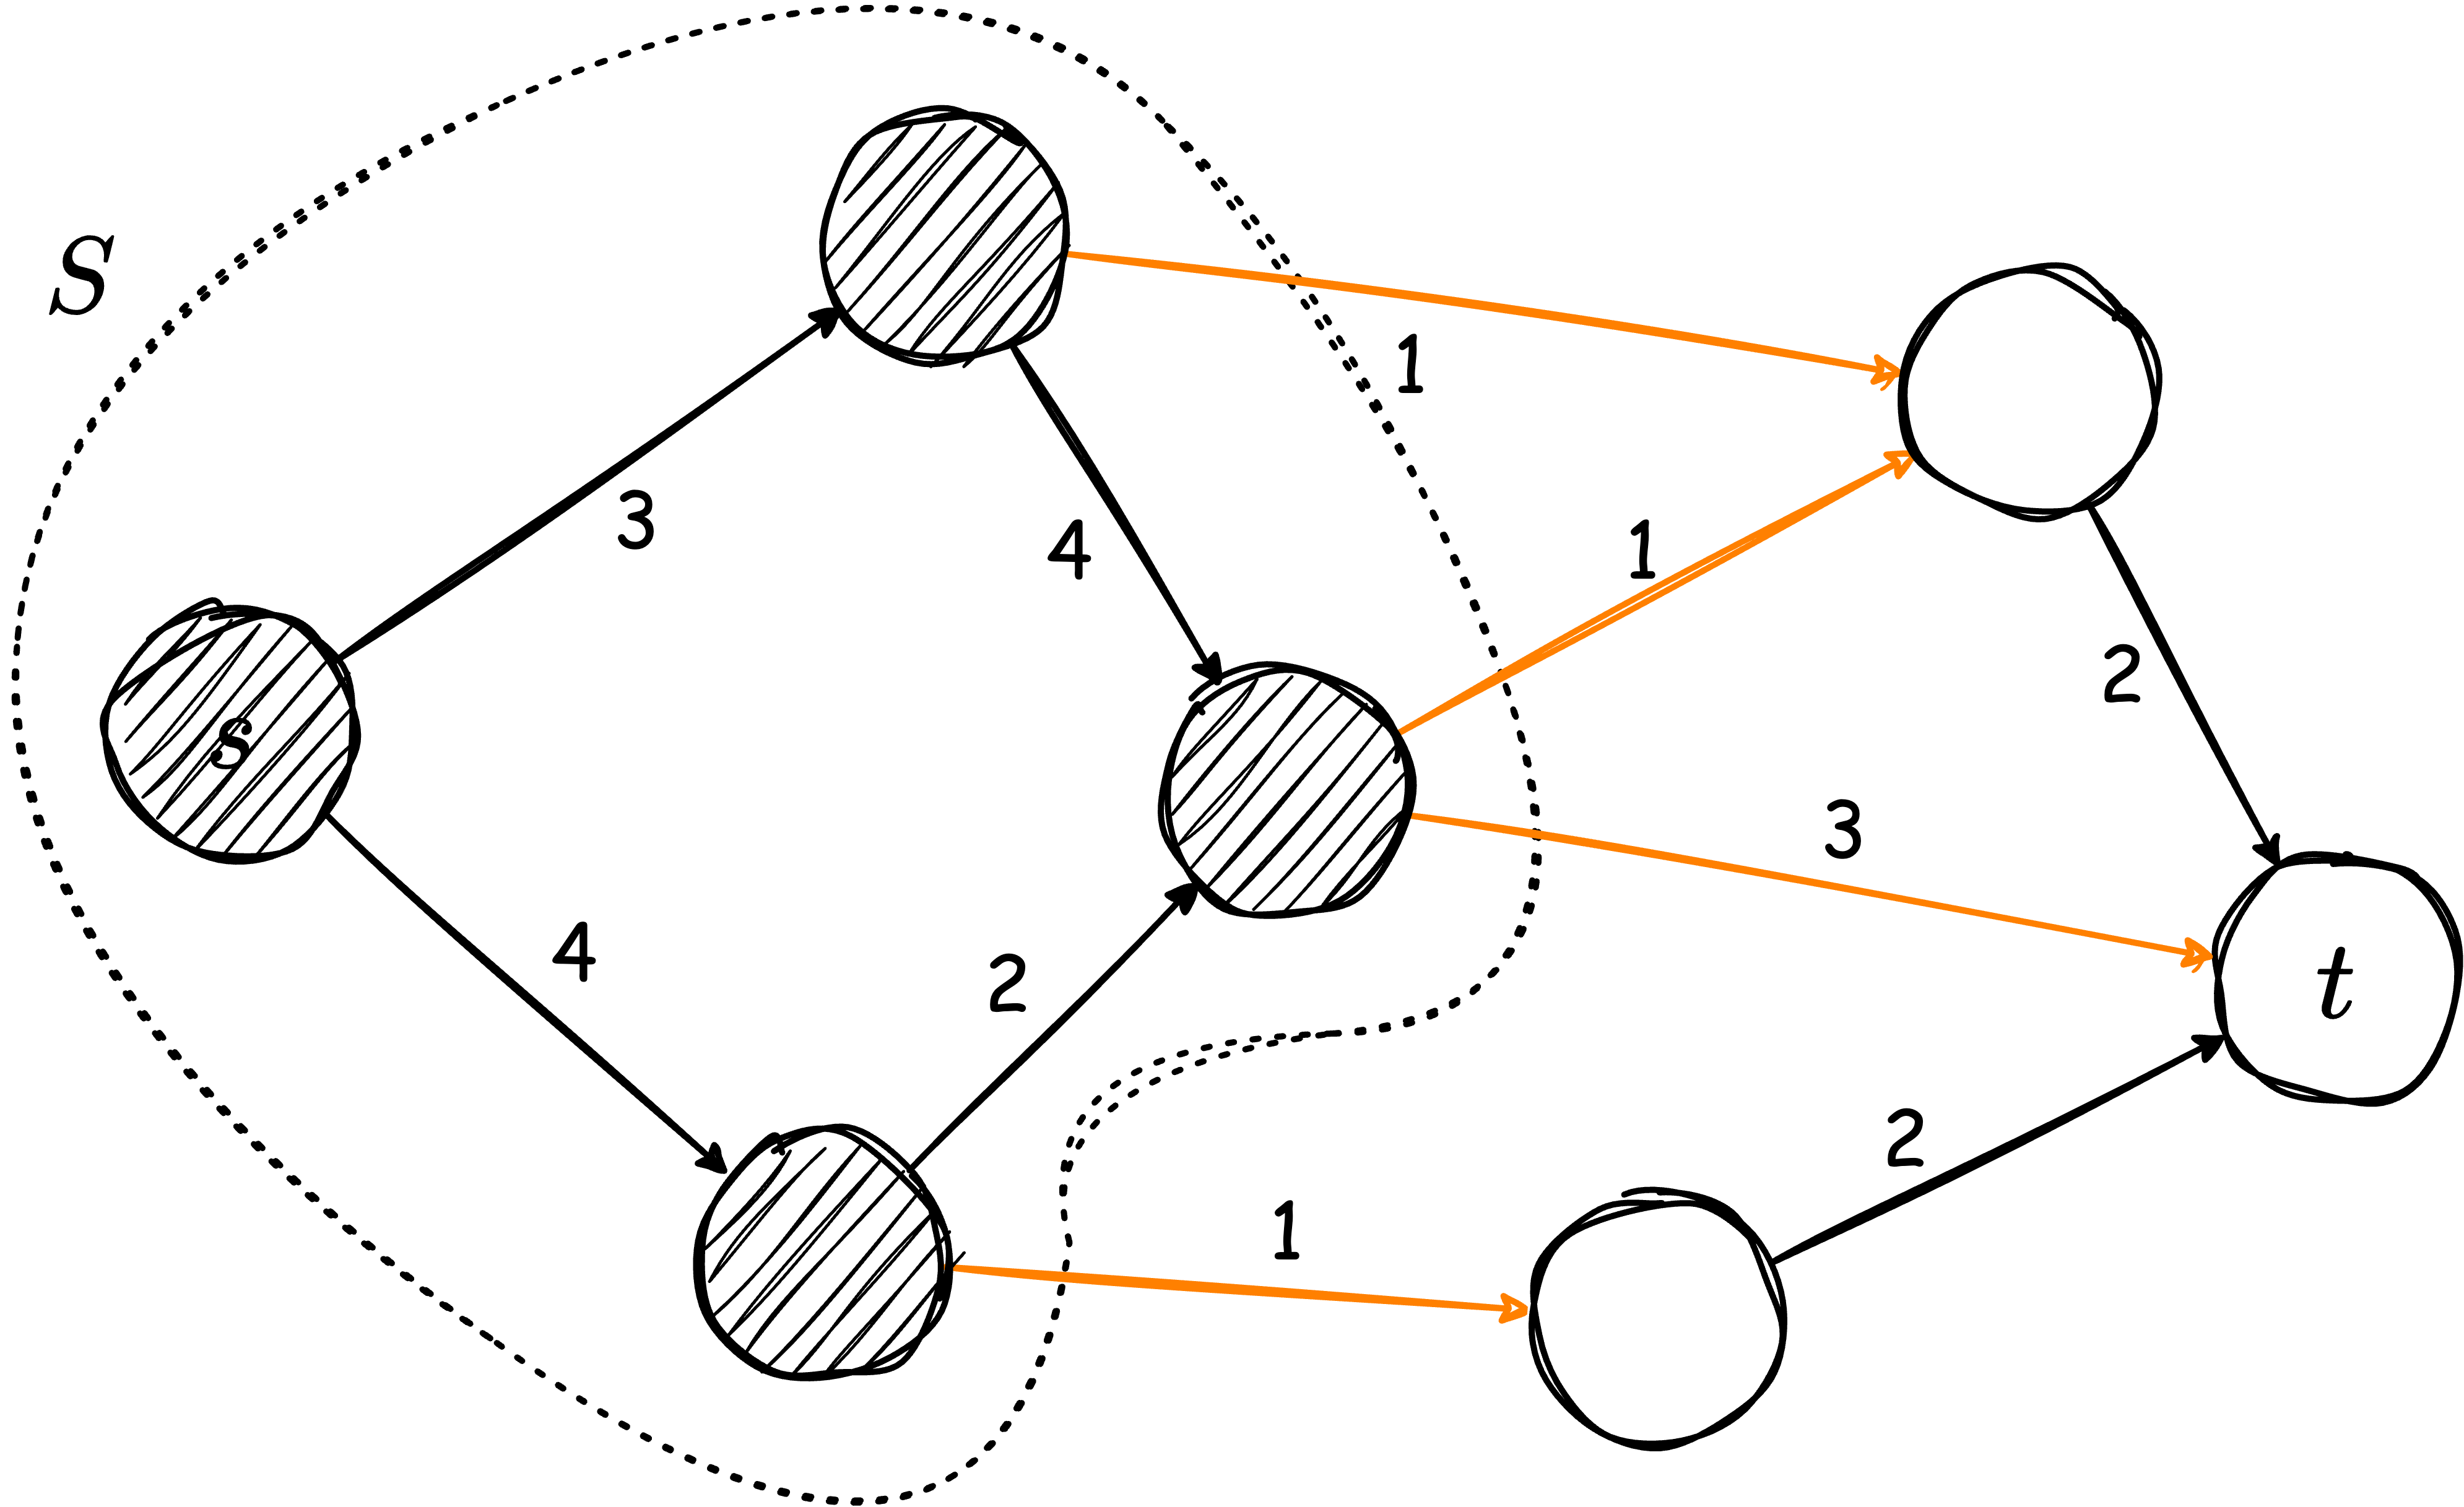
\includegraphics[width=1.0\textwidth]{figures/cut-example.drawio.png}
			\end{figure}
		\end{column}
	\end{columns}
\end{frame}

\begin{frame}{最大フロー問題の定式化\footnote{簡単のため，各 \((i, j) \in E\) について，\(c((i, j)), f((i, j))\) をそれぞれ \(c_{ij}, f_{ij}\) と表記した．}\footnote{第 2 式は，任意の実行可能解において全て等式で成立する（このトリックにより正準形が得られる）．}}
	\begin{itemize}
		\item \(t\) から \(s\) への\alert{容量無限大の仮想辺}を追加し\footnote{\(f_{ts}\) とは異なり，\(c_{ts}\) のような新たな定数を導入するわけではないことに注意する．}，\alert{循環フロー}問題に修正する \\
		      （仮想辺も含めた辺集合について議論する場合には \(E' = E \cup \{(t, s)\}\) を用いる）
	\end{itemize}
	\begin{columns}
		\begin{column}{0.4\textwidth}
			\begin{figure}
				\centering
				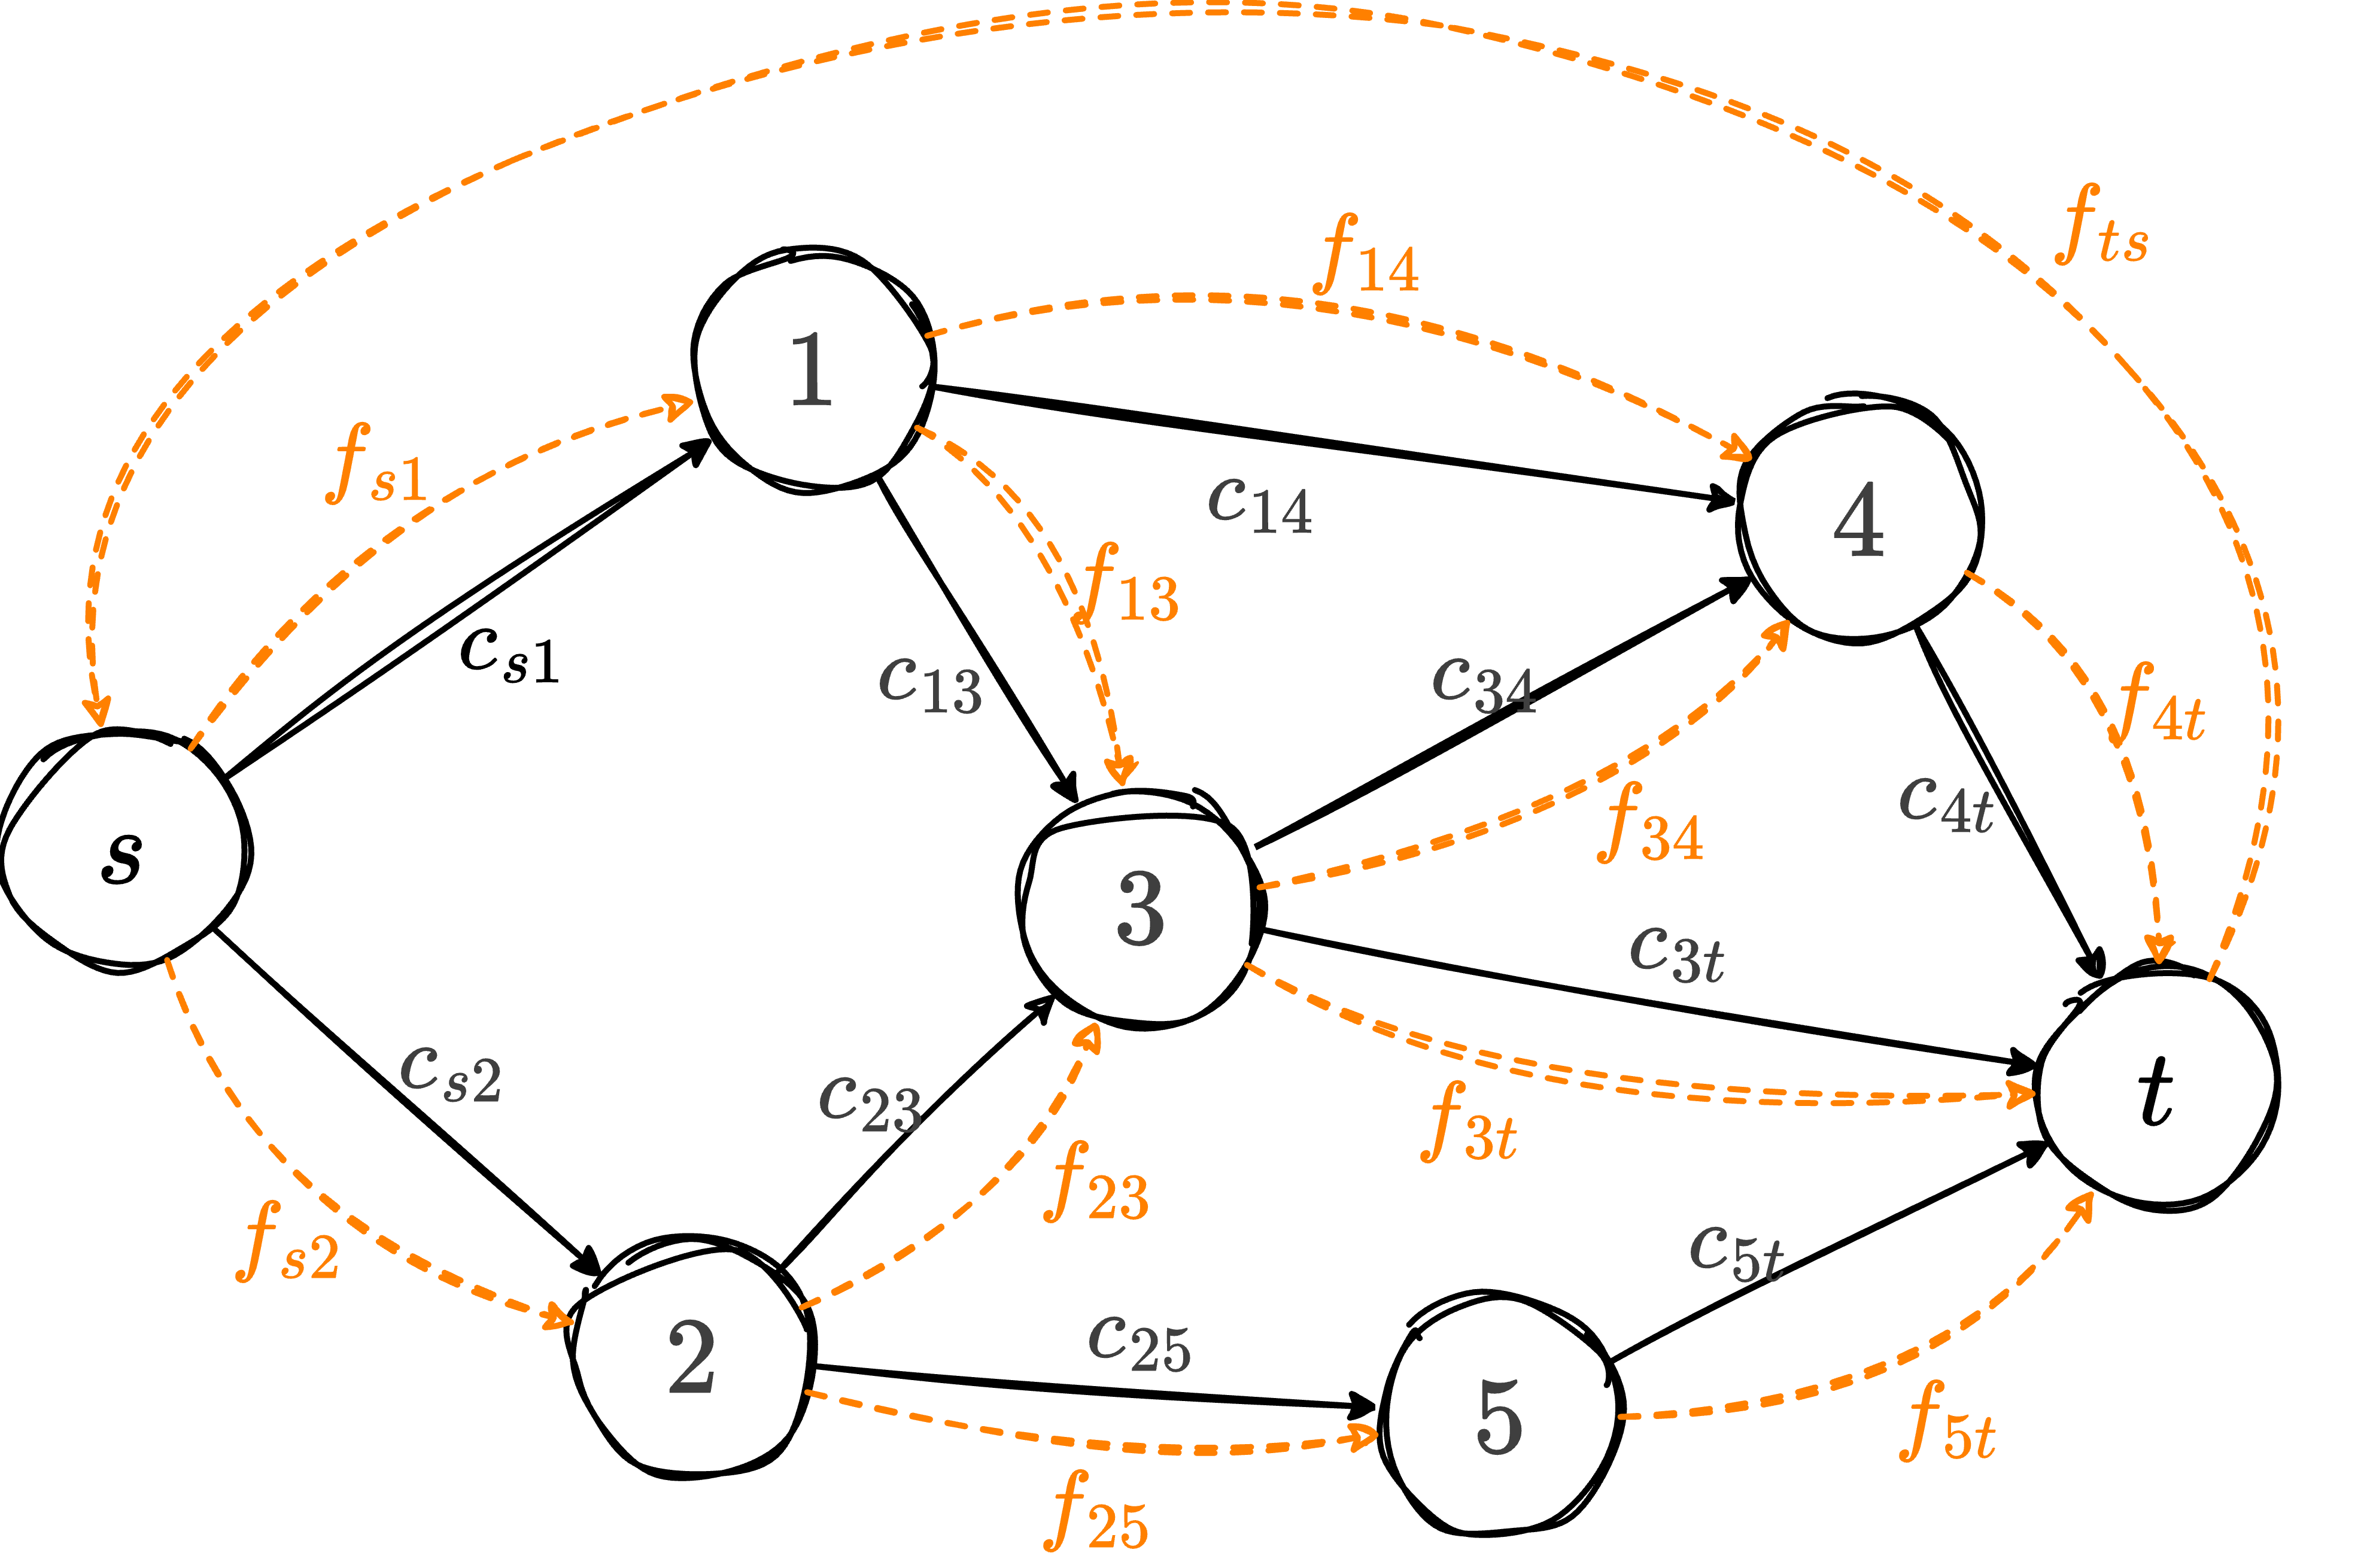
\includegraphics[width=1.0\textwidth]{figures/flow-formulation.drawio.png}
			\end{figure}
		\end{column}
		\begin{column}{0.6\textwidth}
			\small{
				\begin{align*}
					 & \text{max.}   \quad &  & \alert{f_{ts}}                                                                                                         \\
					 & \text{s.t. } \quad  &  & \alert{f_{ij}} \leq c_{ij} \quad                                                            &  & \forall (i, j) \in E  \\
					 &                     &  & \sum_{j: (j, i) \in E'} \alert{f_{ji}} - \sum_{j: (i, j) \in E'} \alert{f_{ij}} \le 0 \quad &  & \forall i \in V       \\
					 &                     &  & \alert{f_{ij}} \geq 0 \quad                                                                 &  & \forall (i, j) \in E'
				\end{align*}
			}
		\end{column}
	\end{columns}
\end{frame}

\begin{frame}{【補足】定式化のトリック}
	\begin{remark}[定式化のトリック]
		次式は任意の実行可能解においてすべて等号で成立する．
		\[\sum_{j: (j, i) \in E'} f_{ji} - \sum_{j: (i, j) \in E'} f_{ij} \le 0 \quad \forall i \in V \tag{*}\]
	\end{remark}

	\vskip -1em

	\small{
		\begin{itemize}
			\item	背理法により示す．ある頂点 \(i'\) で，左辺が右辺より真に小さくなると仮定する \[
				      \sum_{j: (j, i') \in E'} f_{ji'} - \sum_{j: (i', j) \in E'} f_{i'j} < 0
			      \]
			\item 式(*) を各頂点 \(i\) について足し合わせると，\[
				      \sum_{i \in V} \left( \sum_{j: (j, i) \in E'} f_{ji} - \sum_{j: (i, j) \in E'} f_{ij} \right) \alert{< 0}
				      \Leftrightarrow
				      \sum_{(j, i) \in E'} f_{ji} - \sum_{(i, j) \in E'} f_{ij} \alert{< 0}
			      \]
			\item しかし，左辺は常に 0 であるため矛盾が生じる
		\end{itemize}
	}
\end{frame}

\begin{frame}[label=dual-formulation]{最大フロー問題の双対問題}

	\only<1>{
		各辺 \((i, j) \in E\) と各頂点 \(i \in V\) について，双対変数 \(\alert{d_{ij}} (\ge 0), \alert{p_i} (\ge 0)\) を導入する．
		\begin{align*}
			 & \text{max.}   \quad &  & f_{ts}                                                                                                                         \\
			 & \text{s.t. } \quad  &  & f_{ij} \leq c_{ij} \quad                                                    &  & \alert{\times d_{ij}} & \forall (i, j) \in E  \\
			 &                     &  & \sum_{j: (j, i) \in E'} f_{ji} - \sum_{j: (i, j) \in E'} f_{ij} \le 0 \quad &  & \alert{\times p_i}    & \forall i \in V       \\
			 &                     &  & f_{ij} \geq 0 \quad                                                         &  &                       & \forall (i, j) \in E'
		\end{align*}
		\[
			\Downarrow
		\]
		\begin{align*}
			\sum_{(i, j) \in E} c_{ij} \alert{d_{ij}} + \sum_{i \in V} 0 \alert{p_i} & \ge \sum_{(i, j) \in E} f_{ij} \alert{d_{ij}} + \sum_{i \in V} \left( \sum_{j: (j, i) \in E'} f_{ji} - \sum_{j: (i, j) \in E'} f_{ij} \right) \alert{p_i} \\
			                                                                         & = (-\alert{p_t} + \alert{p_s}) \times f_{ts} + \sum_{(i, j) \in E} (\alert{d_{ij}} - \alert{p_i} + \alert{p_j}) \times f_{ij}
		\end{align*}
	}

	\only<2>{
		\begin{align*}
			\sum_{(i, j) \in E} c_{ij} d_{ij} + \sum_{i \in V} 0 p_i & \ge \sum_{(i, j) \in E'} f_{ij} d_{ij} + \sum_{i \in V} \left( \sum_{j: (j, i) \in E'} f_{ji} - \sum_{j: (i, j) \in E} f_{ij} \right) p_i \\
			                                                         & = (-p_t + p_s) \times \alert{f_{ts}} + \sum_{(i, j) \in E} (d_{ij} - p_i + p_j) \times \alert{f_{ij}}
		\end{align*}

		各 \((i, j) \in E'\) について，\(f_{ij} \ge 0\) であるから，次式を満たすとき，
		\begin{align*}
			d_{ij} - p_i + p_j & \ge 0 \quad \forall (i, j) \in E \\
			- p_t + p_s        & \ge 1 \quad
		\end{align*}
		主問題の目的関数 \(f_{ts} (= 1 \times \alert{f_{ts}} + \sum_{(i, j) \in E} 0 \times \alert{f_{ij}})\) の上界が得られる．
	}

	\only<3>{
		よって，
		\begin{align*}
			\text{min.}   \quad & \sum_{(i, j) \in E} c_{ij} d_{ij}                           \\
			\text{s.t.} \quad   & d_{ij} - p_i + p_j \geq 0 \quad   &  & \forall (i, j) \in E \\
			                    & p_s - p_t \geq 1 \quad            &  &                      \\
			                    & d_{ij} \geq 0 \quad               &  & \forall (i, j) \in E \\
			                    & p_i \geq 0 \quad                  &  & \forall i \in V
		\end{align*}
	}
\end{frame}

\begin{frame}{双対問題を直感的に理解する}
	\only<1>{
		双対問題を直感的に理解するために，実数変数を\alert{二値変数}に置き換える．
		\begin{align}
			 & \text{min.}   \quad &  & \sum_{(i, j) \in E} c_{ij} d_{ij}                           \\
			 & \text{s.t.} \quad   &  & d_{ij} - p_i + p_j \geq 0 \quad   &  & \forall (i, j) \in E \\
			 &                     &  & p_s - p_t \geq 1 \quad            &  &                      \\
			 &                     &  & d_{ij} \alert{\in \{0, 1\}} \quad &  & \forall (i, j) \in E \\
			 &                     &  & p_i \alert{\in \{0, 1\}} \quad    &  & \forall i \in V
		\end{align}

		\begin{block}{Observations}
			\begin{itemize}
				\item 目的関数の \(c_{ij}\) は正なので，\alert{\(d_{ij}\) は可能な限り小さく}なるように選ばれる
				\item 式(2) を満たすため \alert{\(d_{ij}\) が 1} になるのは，\alert{\(p_i = 1, p_j = 0\)} のときのみである
				\item 式(3) を満たすのは \alert{\(p_s = 1, p_t = 0\)} のときのみである
			\end{itemize}
		\end{block}
	}

	\only<2>{
		\begin{columns}
			\begin{column}{0.5\textwidth}
				\begin{figure}
					\centering
					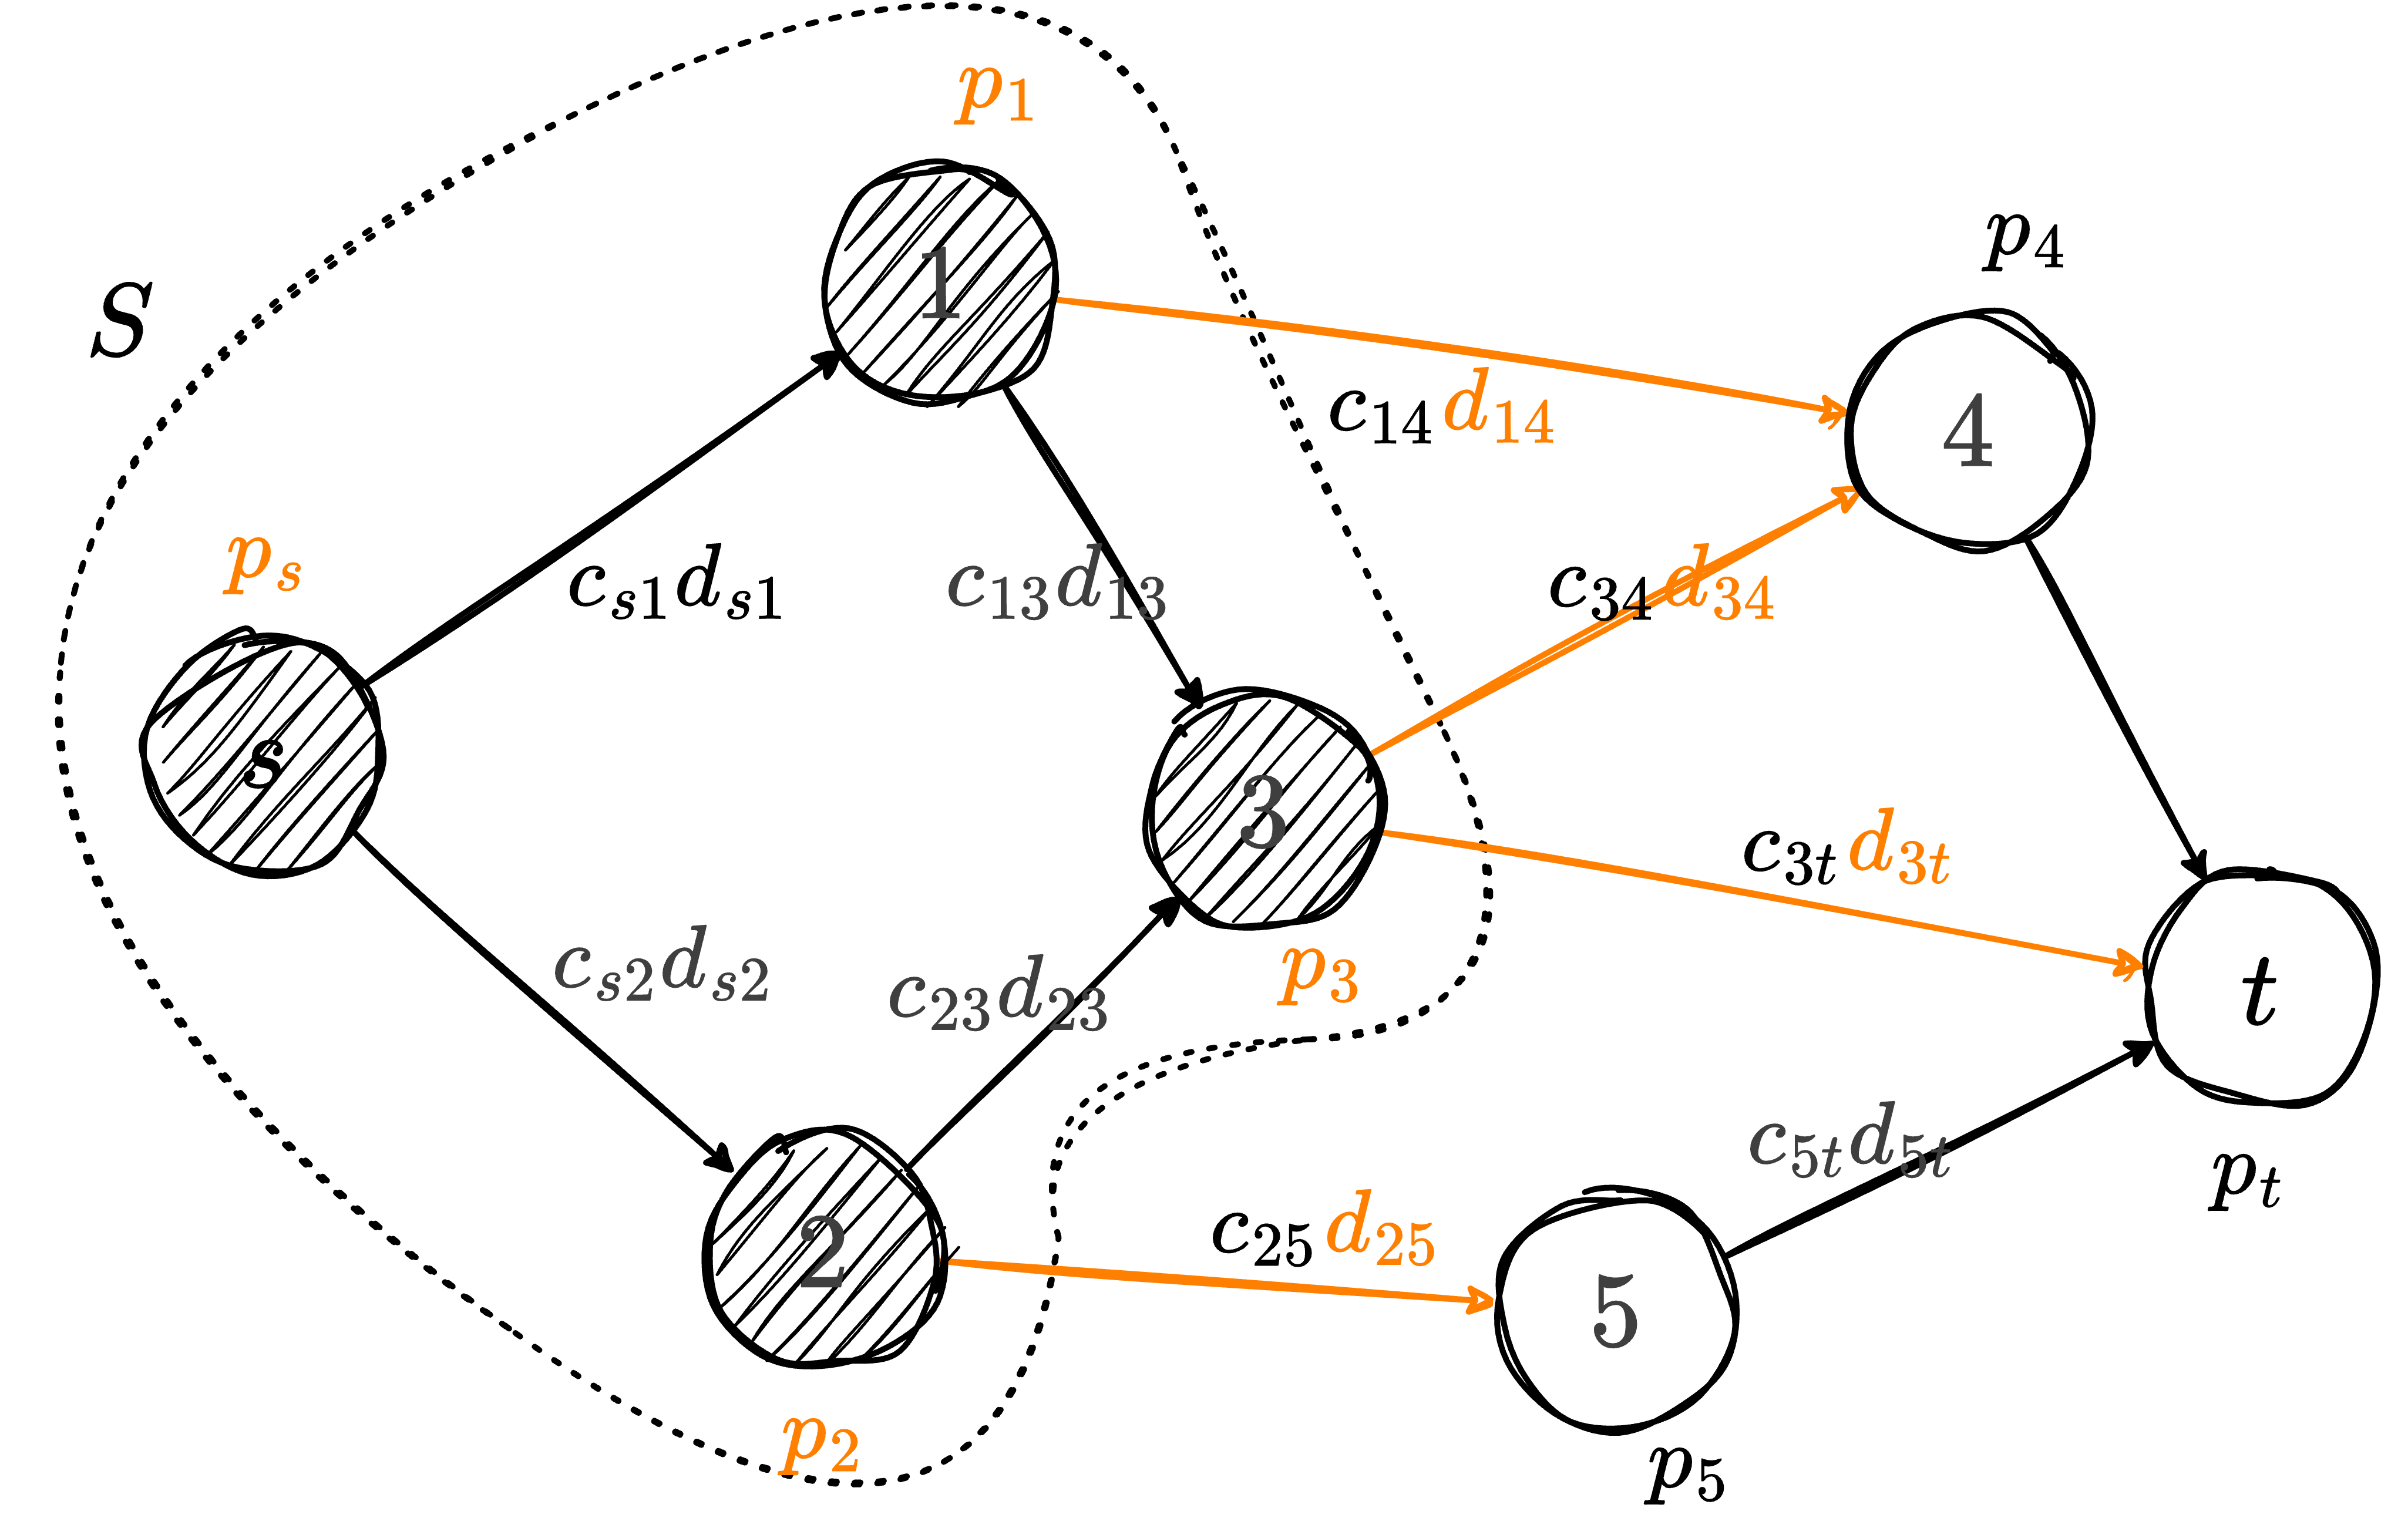
\includegraphics[width=0.9\textwidth]{figures/cut-formulation.drawio.png}
				\end{figure}
			\end{column}
			\begin{column}{0.5\textwidth}
				\small{
					\begin{align*}
						 & \text{min.} \quad &  & \sum_{(i, j) \in E} c_{ij} d_{ij}                           \\
						 & \text{s.t.} \quad &  & d_{ij} - p_i + p_j \geq 0 \quad   &  & \forall (i, j) \in E \\
						 &                   &  & p_s - p_t \geq 1 \quad            &  &                      \\
						 &                   &  & d_{ij} \in \{0, 1\} \quad         &  & \forall (i, j) \in E \\
						 &                   &  & p_i \in \{0, 1\} \quad            &  & \forall i \in V
					\end{align*}
				}
			\end{column}
		\end{columns}

		\vskip 1em

		頂点 \(s\) を含み，頂点 \(t\) を含まない頂点集合 \(S (\subset V\)) に対して，
		\[
			p_i = \begin{cases}
				\alert{1} & \alert{\text{if } i \in S} \\
				0         & \text{otherwise}
			\end{cases}, \quad
			d_{ij} = \begin{cases}
				\alert{1} & \alert{\text{if } i \in S \land j \in V \setminus S} \\
				0         & \text{otherwise}
			\end{cases}
		\]
		となっているから，この整数最適化問題は\alert{最小 s-t カット問題}の定式化である．
	}
\end{frame}

\begin{frame}{では元の双対問題は？}
	\begin{remark}
		最大フロー問題の双対問題は，最小 s-t カット問題の変数の整数制約と上界制約を除去した緩和問題とみなせる．
	\end{remark}

	TODO: 時間があればあとでやる．
\end{frame}

\begin{frame}{ここまでのまとめ}
	\begin{figure}
		\centering
		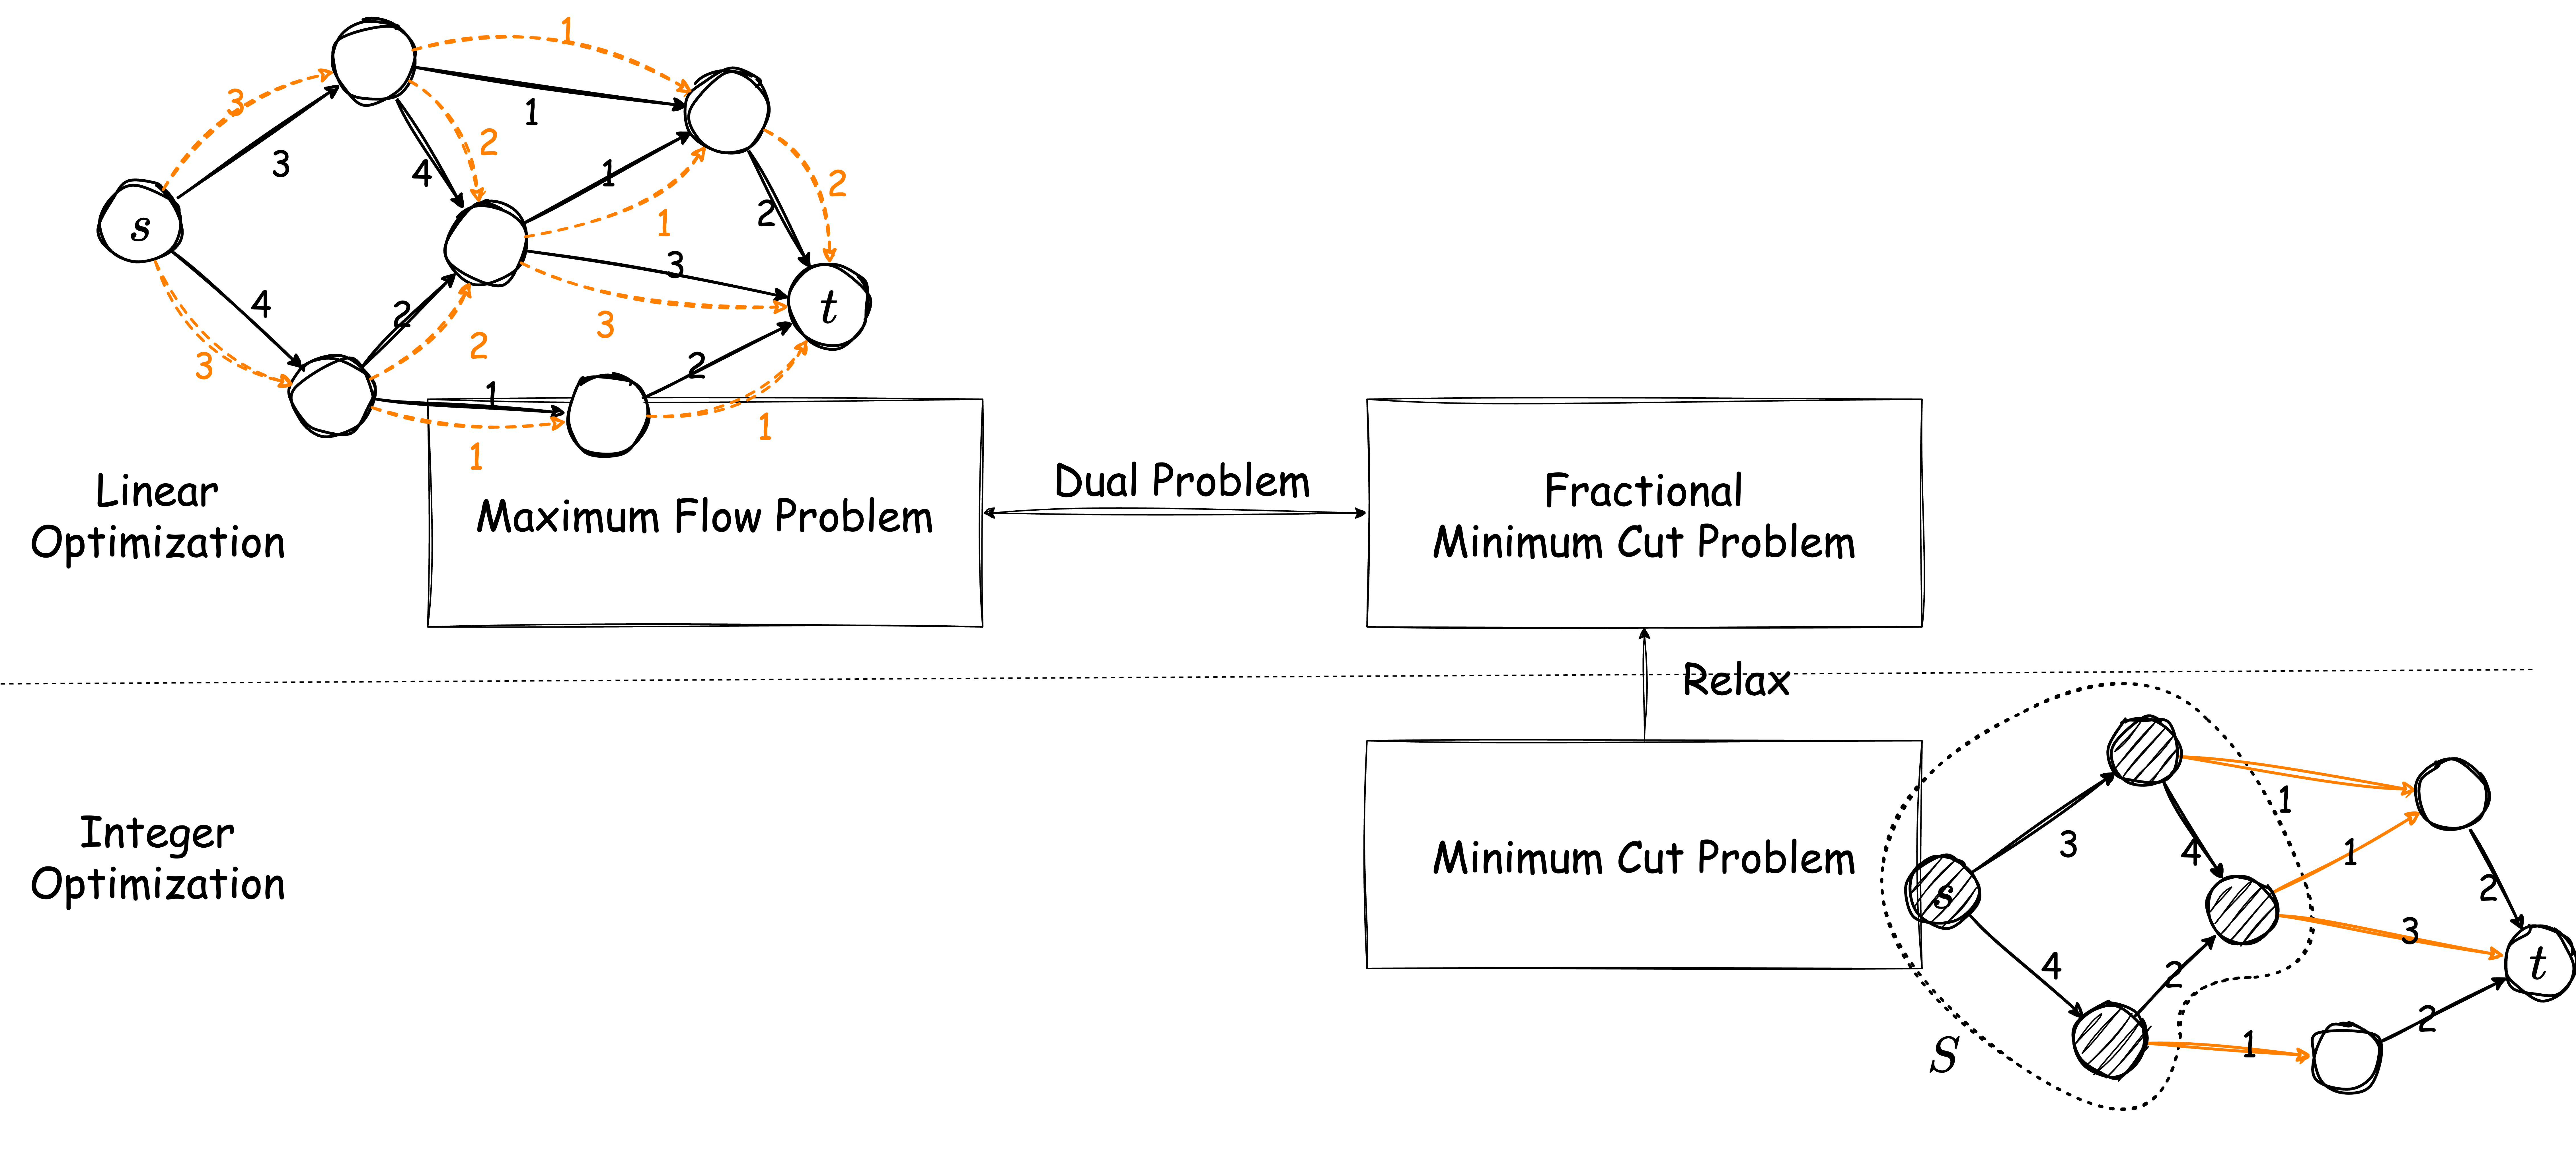
\includegraphics[width=0.8\textwidth]{figures/overview.drawio.png}
	\end{figure}

	これらの値の大小関係は？？？
\end{frame}

\againframe<3>{dual-formulation}

\begin{frame}{小数版カット問題の行列表現}
	\begin{columns}
		\begin{column}{0.4\textwidth}
			\begin{align*}
				d_{ij} - p_i + p_j & \geq 0 & \forall (i, j) \in E \\
				p_s - p_t          & \geq 1 &                      \\
				d_{ij}             & \geq 0 & \forall (i, j) \in E \\
				p_i                & \geq 0 & \forall i \in V
			\end{align*}
		\end{column}
		\begin{column}{0.5\textwidth}
			\begin{figure}
				\centering
				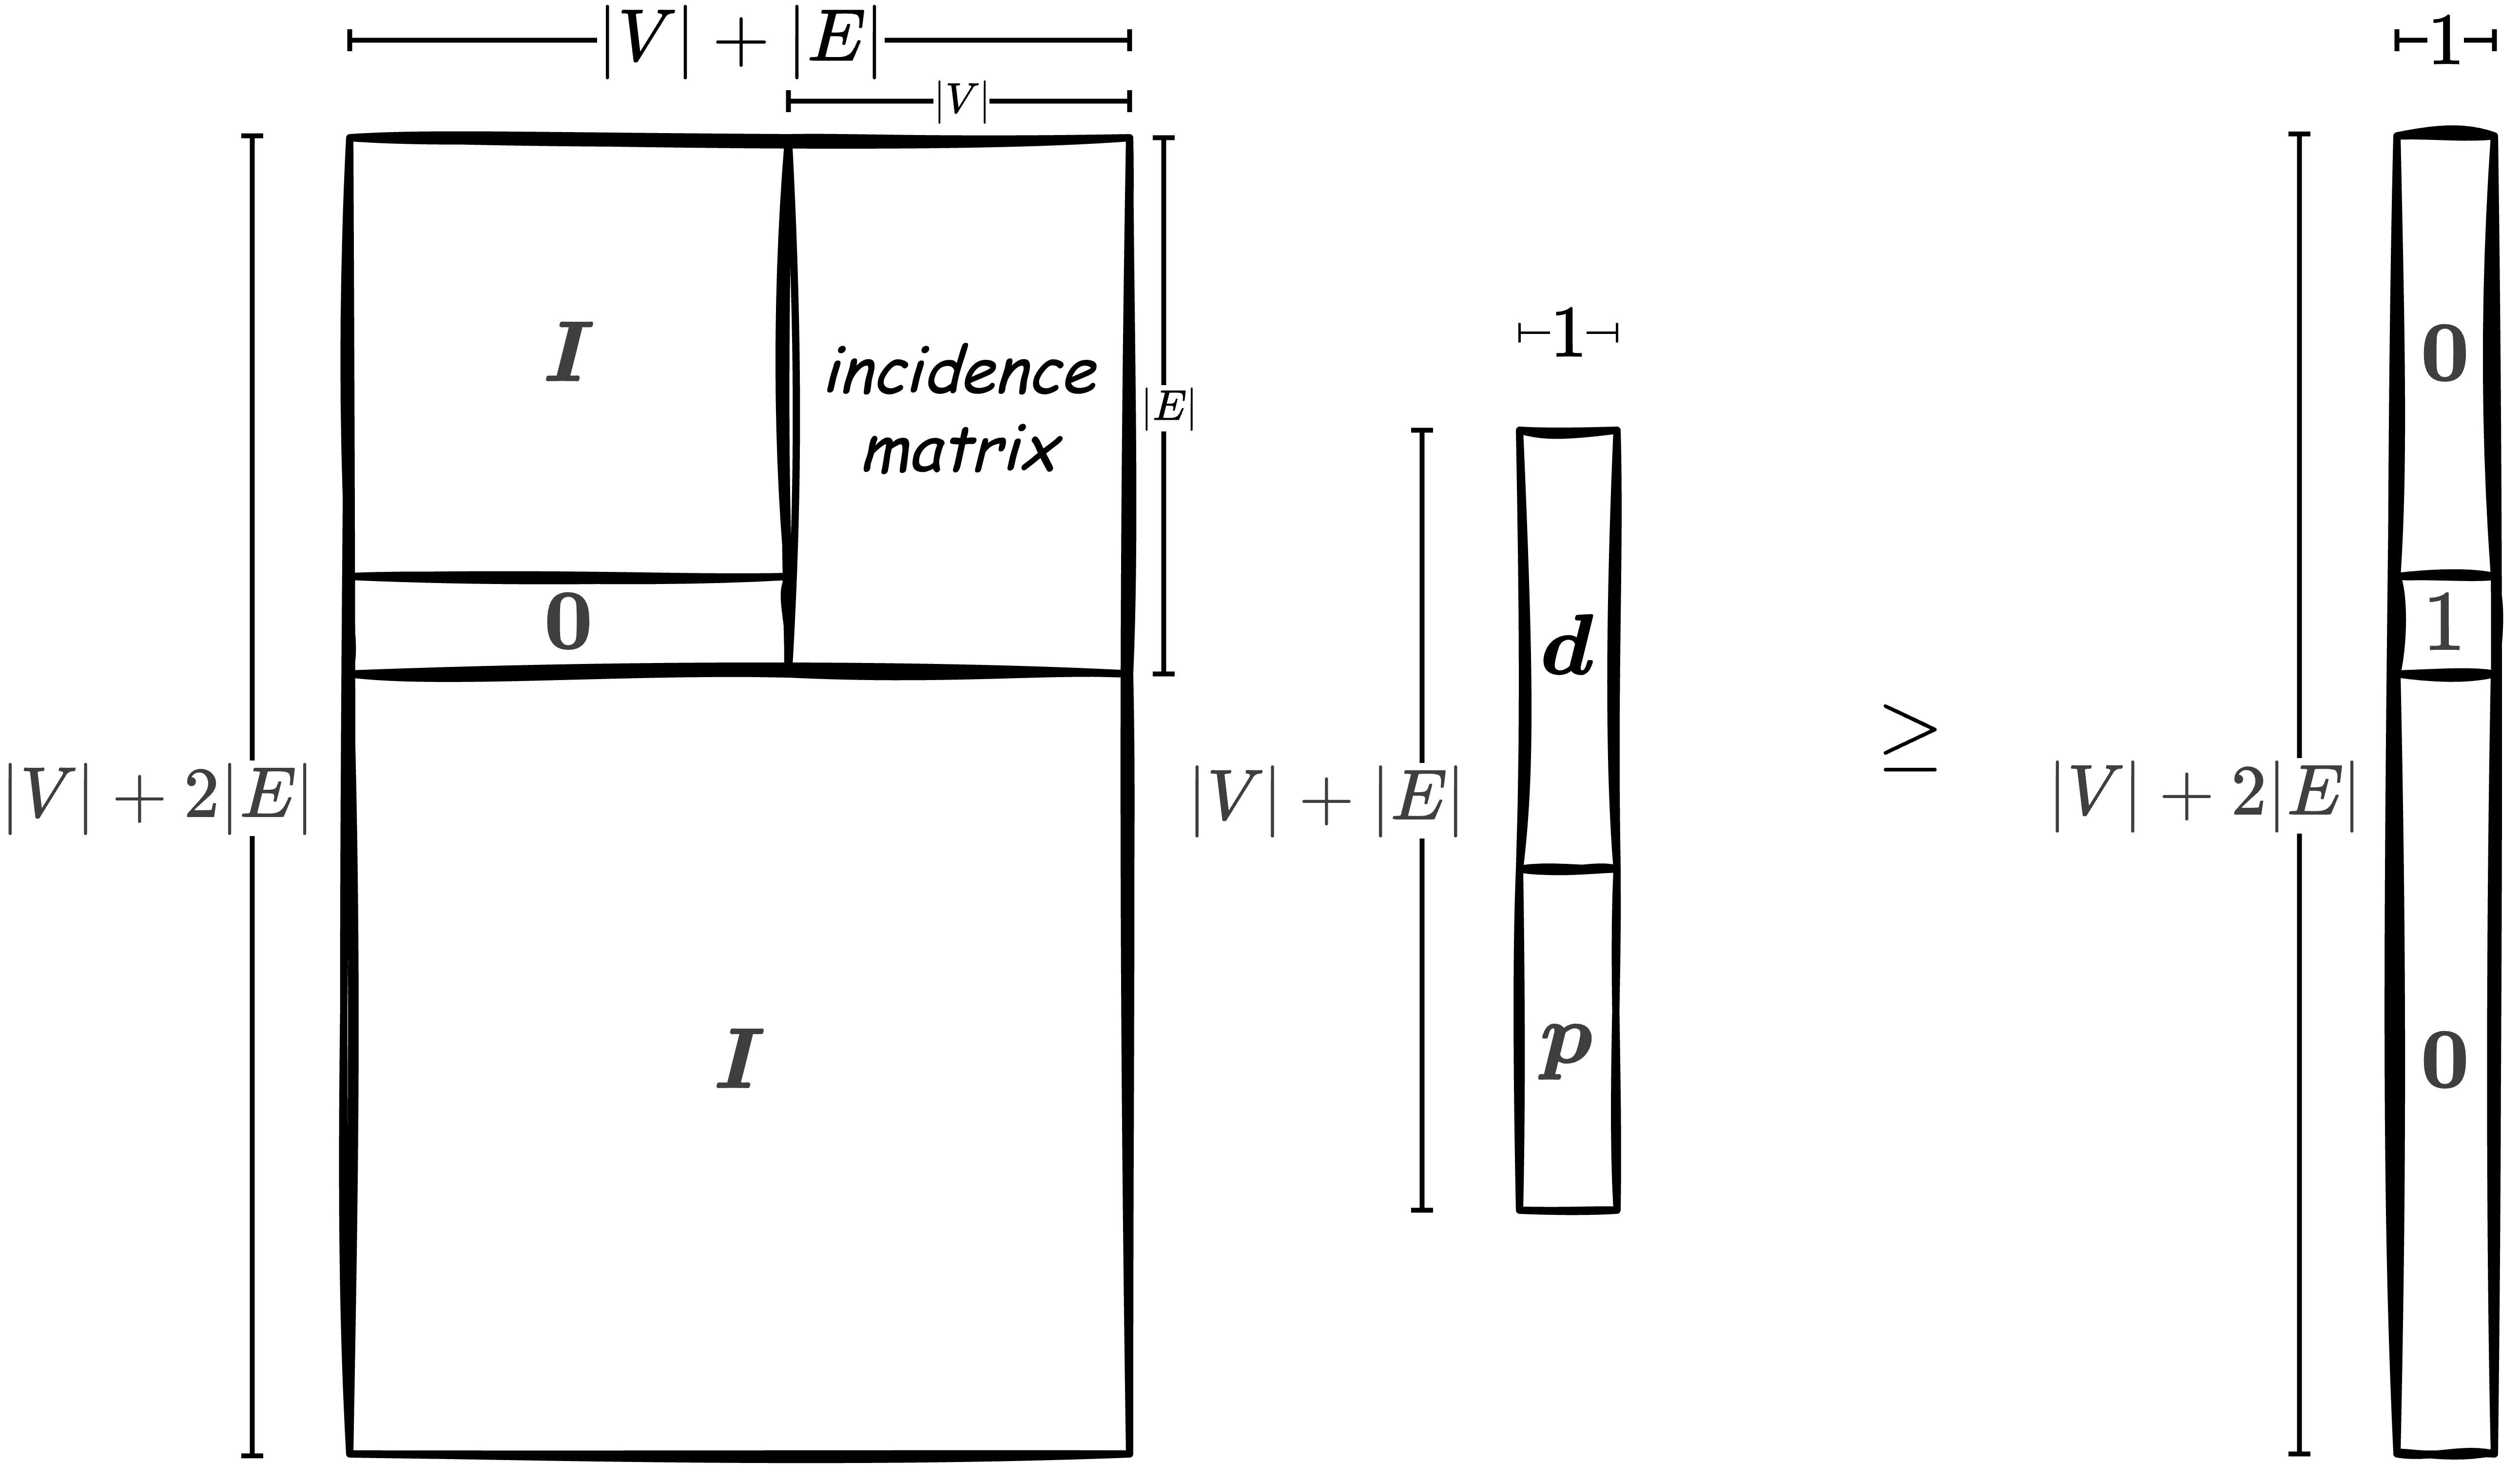
\includegraphics[width=1.0\textwidth]{figures/cut-matrix.drawio.png}
			\end{figure}
		\end{column}
	\end{columns}
\end{frame}

\begin{frame}{完全単模行列}
	\begin{definition}[完全単模行列]
		整数行列 \(A \in \mathbb{Z}^{m \times n}\) が\alert{完全単模行列}であるとは，\(A\) の任意の正方部分行列の行列式が \(0, +1, -1\) のいずれかであることをいう．
	\end{definition}

	\begin{example}[完全単模行列の例]
		\[
			\begin{pmatrix}
				1 & 0 & 0 & 0 \\
				0 & 1 & 0 & 0 \\
				0 & 0 & 1 & 0 \\
				0 & 0 & 0 & 1 \\
			\end{pmatrix},
			\begin{pmatrix}
				-1 & -1 & 0  & 0  & 0  & 1  \\
				1  & 0  & -1 & -1 & 0  & 0  \\
				0  & 1  & 1  & 0  & -1 & 0  \\
				0  & 0  & 0  & 1  & 1  & -1 \\
			\end{pmatrix},
			\begin{pmatrix}
				1 & 0 & 0 & 0 & 1 \\
				0 & 1 & 0 & 1 & 0 \\
				0 & 1 & 0 & 0 & 1 \\
				0 & 0 & 1 & 1 & 0 \\
			\end{pmatrix}
		\] はいずれも完全単模行列である．
	\end{example}
\end{frame}

\begin{frame}{完全単模行列の性質}
	\begin{lemma}[完全単模行列の性質]
		行列 \(A \in \mathbb{Z}^{m \times n}\) が完全単模行列であるとき，次が成り立つ．
		\begin{enumerate}
			\item \(-A\) は完全単模行列である．
			\item \(A^{\top}\) は完全単模行列である．
			\item 任意の単位行列 \(I\) を \(A\) の任意の列に追加して得られる行列 \([A \mid I]\) は完全単模行列である．
		\end{enumerate}
	\end{lemma}
	\begin{lemma}[有向グラフの接続行列の完全単模性]
		任意の有向グラフに対する\alert{接続行列は完全単模行列}である．
	\end{lemma}
\end{frame}

\begin{frame}{接続行列の完全単模性}
	\begin{lemma*}[有向グラフの接続行列の完全単模性]
		任意の\alert{有向グラフ}に対する\alert{接続行列は完全単模行列}である．
	\end{lemma*}

	\textbf{Proof.}
	\(k\) 次正方部分行列を考え，\(k\) に対する数学的帰納法で示す．

	\textbf{Base case: }
	\(1\) 次正方部分行列の行列式は \(0, +1, -1\) のいずれかである．

	\textbf{Induction step: }
	\alert{\(k\) 次正方部分行列の行列式は \(0, +1, -1\) のいずれかであると仮定}し，\(k + 1\) 次正方部分行列 \(B\) を考える．
	\begin{itemize}
		\item \(B\) に零行が含まれる場合，\(\det(B) = 0\)
		\item \(B\) に 1 個の非零要素を持つ行が含まれる場合，その要素を含む行で展開して，帰納法の仮定より \(\det(B) = 0, +1, -1\)
		\item それ以外の場合，\(B\) の各行は 2 個の非零要素を持つ．
		      このとき，\(B\) の行ベクトルは線形従属であるため，\(\det(B) = 0\)
	\end{itemize}
	\qed

\end{frame}

\begin{frame}{完全単模行列における線形最適化問題の解の整数性}
	\begin{theorem}[線形計画法の基本定理~\cite{bertsekas1995nonlinear}] %\label{thm:fundamental-theorem-of-linear-programming}
		\(P\) を \(\mathbb{R}^n\) 上の凸多面体とし，1 つ以上の頂点を持つと仮定する．
		このとき，ある線形関数が \(P\) 上で\alert{最小値}を取るならば，その値は \(P\) の\alert{頂点}のうちの 1 つで達成される．
	\end{theorem}

	\begin{theorem}[Hoffman-Kruskal の定理~\cite{hoffman2010integral}]
		ある整数行列 \(A \in \mathbb{Z}^{m \times n}\) が\alert{完全単模行列}であるならば\footnote{なお実際のところ \cite{hoffman2010integral} では，必要十分条件であることが示されている．}，
		任意の \(\boldsymbol{b} \in \mathbb{Z}^m\) に対する，多面体 \(\{ \boldsymbol{x} \in \mathbb{R}^n \mid A \boldsymbol{x} \le \boldsymbol{b}, \boldsymbol{x} \ge 0\}\) の頂点は\alert{整数ベクトル}である．
	\end{theorem}

	\only<1>{
		\begin{columns}
			\begin{column}{0.5\textwidth}
				\begin{figure}
					\centering
					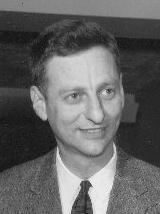
\includegraphics[width=0.22\textwidth]{figures/alan-j-hoffman.jpeg}
					\caption{Alan Jerome Hoffman (1924-2021)}
				\end{figure}
			\end{column}
			\begin{column}{0.5\textwidth}
				\begin{figure}
					\centering
					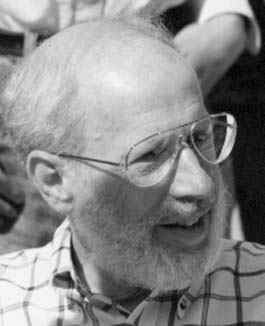
\includegraphics[width=0.25\textwidth]{figures/joseph-b-kruskal.jpeg}
					\caption{Joseph Bernard Kruskal (1928-2010)}
				\end{figure}
			\end{column}
		\end{columns}
	}
	\only<2>{
		\begin{corollary}[完全単模行列における線形最適化問題の解の整数性]
			\(m \times n\) 行列 \(A\) が完全単模行列であり，\(\boldsymbol{b} \in \mathbb{Z}^m\) であれば，線形最適化問題 \[
				\text{min.} \quad \boldsymbol{c}^{\top} \boldsymbol{x} \quad \text{s.t.} \quad A \boldsymbol{x} \le \boldsymbol{b}, \boldsymbol{x} \ge 0
			\] は\alert{整数最適解}を持つ．
		\end{corollary}
	}
\end{frame}

\begin{frame}{線形計画法の基本定理~\cite{bertsekas1995nonlinear} の証明}
	\begin{theorem*}[線形計画法の基本定理~\cite{bertsekas1995nonlinear}]
		\(P\) を \(\mathbb{R}^n\) 上の凸多面体とし，1 つ以上の頂点を持つと仮定する．
		このとき，ある線形関数が \(P\) 上で\alert{最小値}を取るならば，その値は \(P\) の\alert{頂点}のうちの 1 つで達成される．
	\end{theorem*}

	\small{
	\only<1>{
		\textbf{Proof.}
		線形関数を \(f(\boldsymbol{x}) = \boldsymbol{c}^{\top} \boldsymbol{x}\) とし，最小値を達成する解のひとつを \(\boldsymbol{x}^*\) とする．

		\structure{まず，\alert{\(\boldsymbol{x}^*\) が \(P\) の境界上に存在する}ことを背理法により示す．}

		\(\boldsymbol{x}^* \in \interior (P)\) を仮定する．このとき，ある \(\epsilon > 0\) が存在して，半径 \(\epsilon\) の開球 \(B(\boldsymbol{x}^*, \epsilon)\) が \(P\) に含まれる．
		それゆえ，\[\boldsymbol{x}^* - \frac{\epsilon}{2}\frac{\boldsymbol{c}}{||\boldsymbol{c}||} \in P\]
		かつ \[f \left(\boldsymbol{x}^* - \frac{\epsilon}{2}\frac{\boldsymbol{c}}{||\boldsymbol{c}||} \right)
			= \boldsymbol{c}^{\top} \left( \boldsymbol{x}^* - \frac{\epsilon}{2}\frac{\boldsymbol{c}}{||\boldsymbol{c}||} \right)
			= \boldsymbol{c}^{\top} \boldsymbol{x}^* - \frac{\epsilon}{2} \frac{\boldsymbol{c}^{\top} \boldsymbol{c}}{||\boldsymbol{c}||}
			= \boldsymbol{c}^{\top} \boldsymbol{x}^* - \frac{\epsilon}{2} ||\boldsymbol{c}|| < \boldsymbol{c}^{\top} \boldsymbol{x}^*\]
		がいえるため，\alert{\(\boldsymbol{c}^{\top}\boldsymbol{x}^*\) の最小性に矛盾}する．
	}

	\only<2>{
	\structure{次に，\(\boldsymbol{x}^*\) が \(P\) の頂点でないと仮定する．}

	\(P\) の凸性から，\(x^*\) は \(P\) の頂点 \(\boldsymbol{v}_1, \boldsymbol{v}_2, \ldots, \boldsymbol{v}_k\) の凸結合として表される．すなわち，
	\[\boldsymbol{x}^* = \sum_{i=1}^{k} \lambda_i \boldsymbol{v}_i, \quad \sum_{i=1}^{k} \lambda_i = 1, \quad \lambda_i \geq 0 \quad \forall i\]

	このとき，\[
		0 = f\left( \sum_{i=1}^{k} \lambda_i \boldsymbol{v}_i - \boldsymbol{x}^* \right) \underbrace{=}_{\mathclap{\raisebox{-1.5em}{linearity of \(f\)}}}
		\left( \sum_{i=1}^{k} \lambda_i f(\boldsymbol{v}_i) \right) - f(\boldsymbol{x}^*) \underbrace{=}_{\mathclap{\raisebox{-1.5em}{\(\sum_{i=1}^{k} \lambda_i = 1\)}}}
		\sum_{i=1}^{k} \lambda_i \left( f(\boldsymbol{v}_i) - f(\boldsymbol{x}^*) \right)
	\]
	}

	\only<3>{
		\[
			\sum_{i=1}^{k} \lambda_i \left( f(\boldsymbol{v}_i) - f(\boldsymbol{x}^*) \right) = 0
		\]

		\(\lambda_i \geq 0\) かつ \(f(\boldsymbol{v}_i) - f(\boldsymbol{x}^*) \geq 0\) であるため\footnote{\(f(\boldsymbol{x}^*)\) は最小値．}，
		\(\lambda_i > 0\) ならば \(f(\boldsymbol{v}_i) - f(\boldsymbol{x}^*) = 0\) でなければならない．
		したがって，\(\lambda_i > 0\) なる \(i\) に対して，\(f(\boldsymbol{v}_i) = f(\boldsymbol{x}^*)\) が成立する\footnote{\(\sum_{i=1}^{k} \lambda_i = 1\) より，そのような \(\lambda_i\) が少なくとも 1 つは存在する．}．

		ゆえに，\(P\) の頂点のうち，最小値を取る点が少なくとも 1 つ存在する．\qed
	}
	}

\end{frame}

\begin{frame}{Hoffman-Kruskal の定理~\cite{hoffman2010integral} の証明}
	\begin{theorem*}[Hoffman-Kruskal の定理~\cite{hoffman2010integral}]
		ある整数行列 \(A \in \mathbb{Z}^{m \times n}\) が\alert{完全単模行列}であるならば，
		任意の \(\boldsymbol{b} \in \mathbb{Z}^m\) に対する，多面体 \(P = \{ \boldsymbol{x} \in \mathbb{R}^n \mid A \boldsymbol{x} \le \boldsymbol{b}, \boldsymbol{x} \ge \boldsymbol{0}\}\) の頂点は\alert{整数ベクトル}である．
	\end{theorem*}

	\small{
		\textbf{Proof.}
		多面体の任意の頂点 \(x'\) は，行列 \([A; I]\) の \(n\) 個の線形独立な行ベクトルからなる部分行列 \(A'\) と，それに対応する \([\boldsymbol{b}; \boldsymbol{0}]\) の成分からなるベクトル \(\boldsymbol{b}'\) を用いて，
		\[A'\boldsymbol{x}' = \boldsymbol{b}' \Leftrightarrow \boldsymbol{x}' = (A')^{-1} \boldsymbol{b}'\] と表される．
		クラメールの公式によれば，\((A')^{-1}\) の各成分は，\[(A')^{-1} = \frac{\mathrm{adj}(A')}{\det(A')}\] より整数である．
		よって，\(\boldsymbol{b}'\) の各成分が整数であることから，\(\boldsymbol{x}'\) の各成分も整数である．\qed
	}

\end{frame}



\begin{frame}[standout]
	Coffee Break
\end{frame}

\begin{frame}{最大マッチングと最小点カバー}

	\vskip 1em

	\begin{corollary}[Konig の定理] % Kőnig's theorem
		任意の二部グラフにおいて，\alert{最大マッチング}のサイズは\alert{最小点カバー}のサイズに等しい．
	\end{corollary}

	\only<1>{
		\begin{columns}
			\begin{column}{0.5\textwidth}
				\begin{figure}
					\centering
					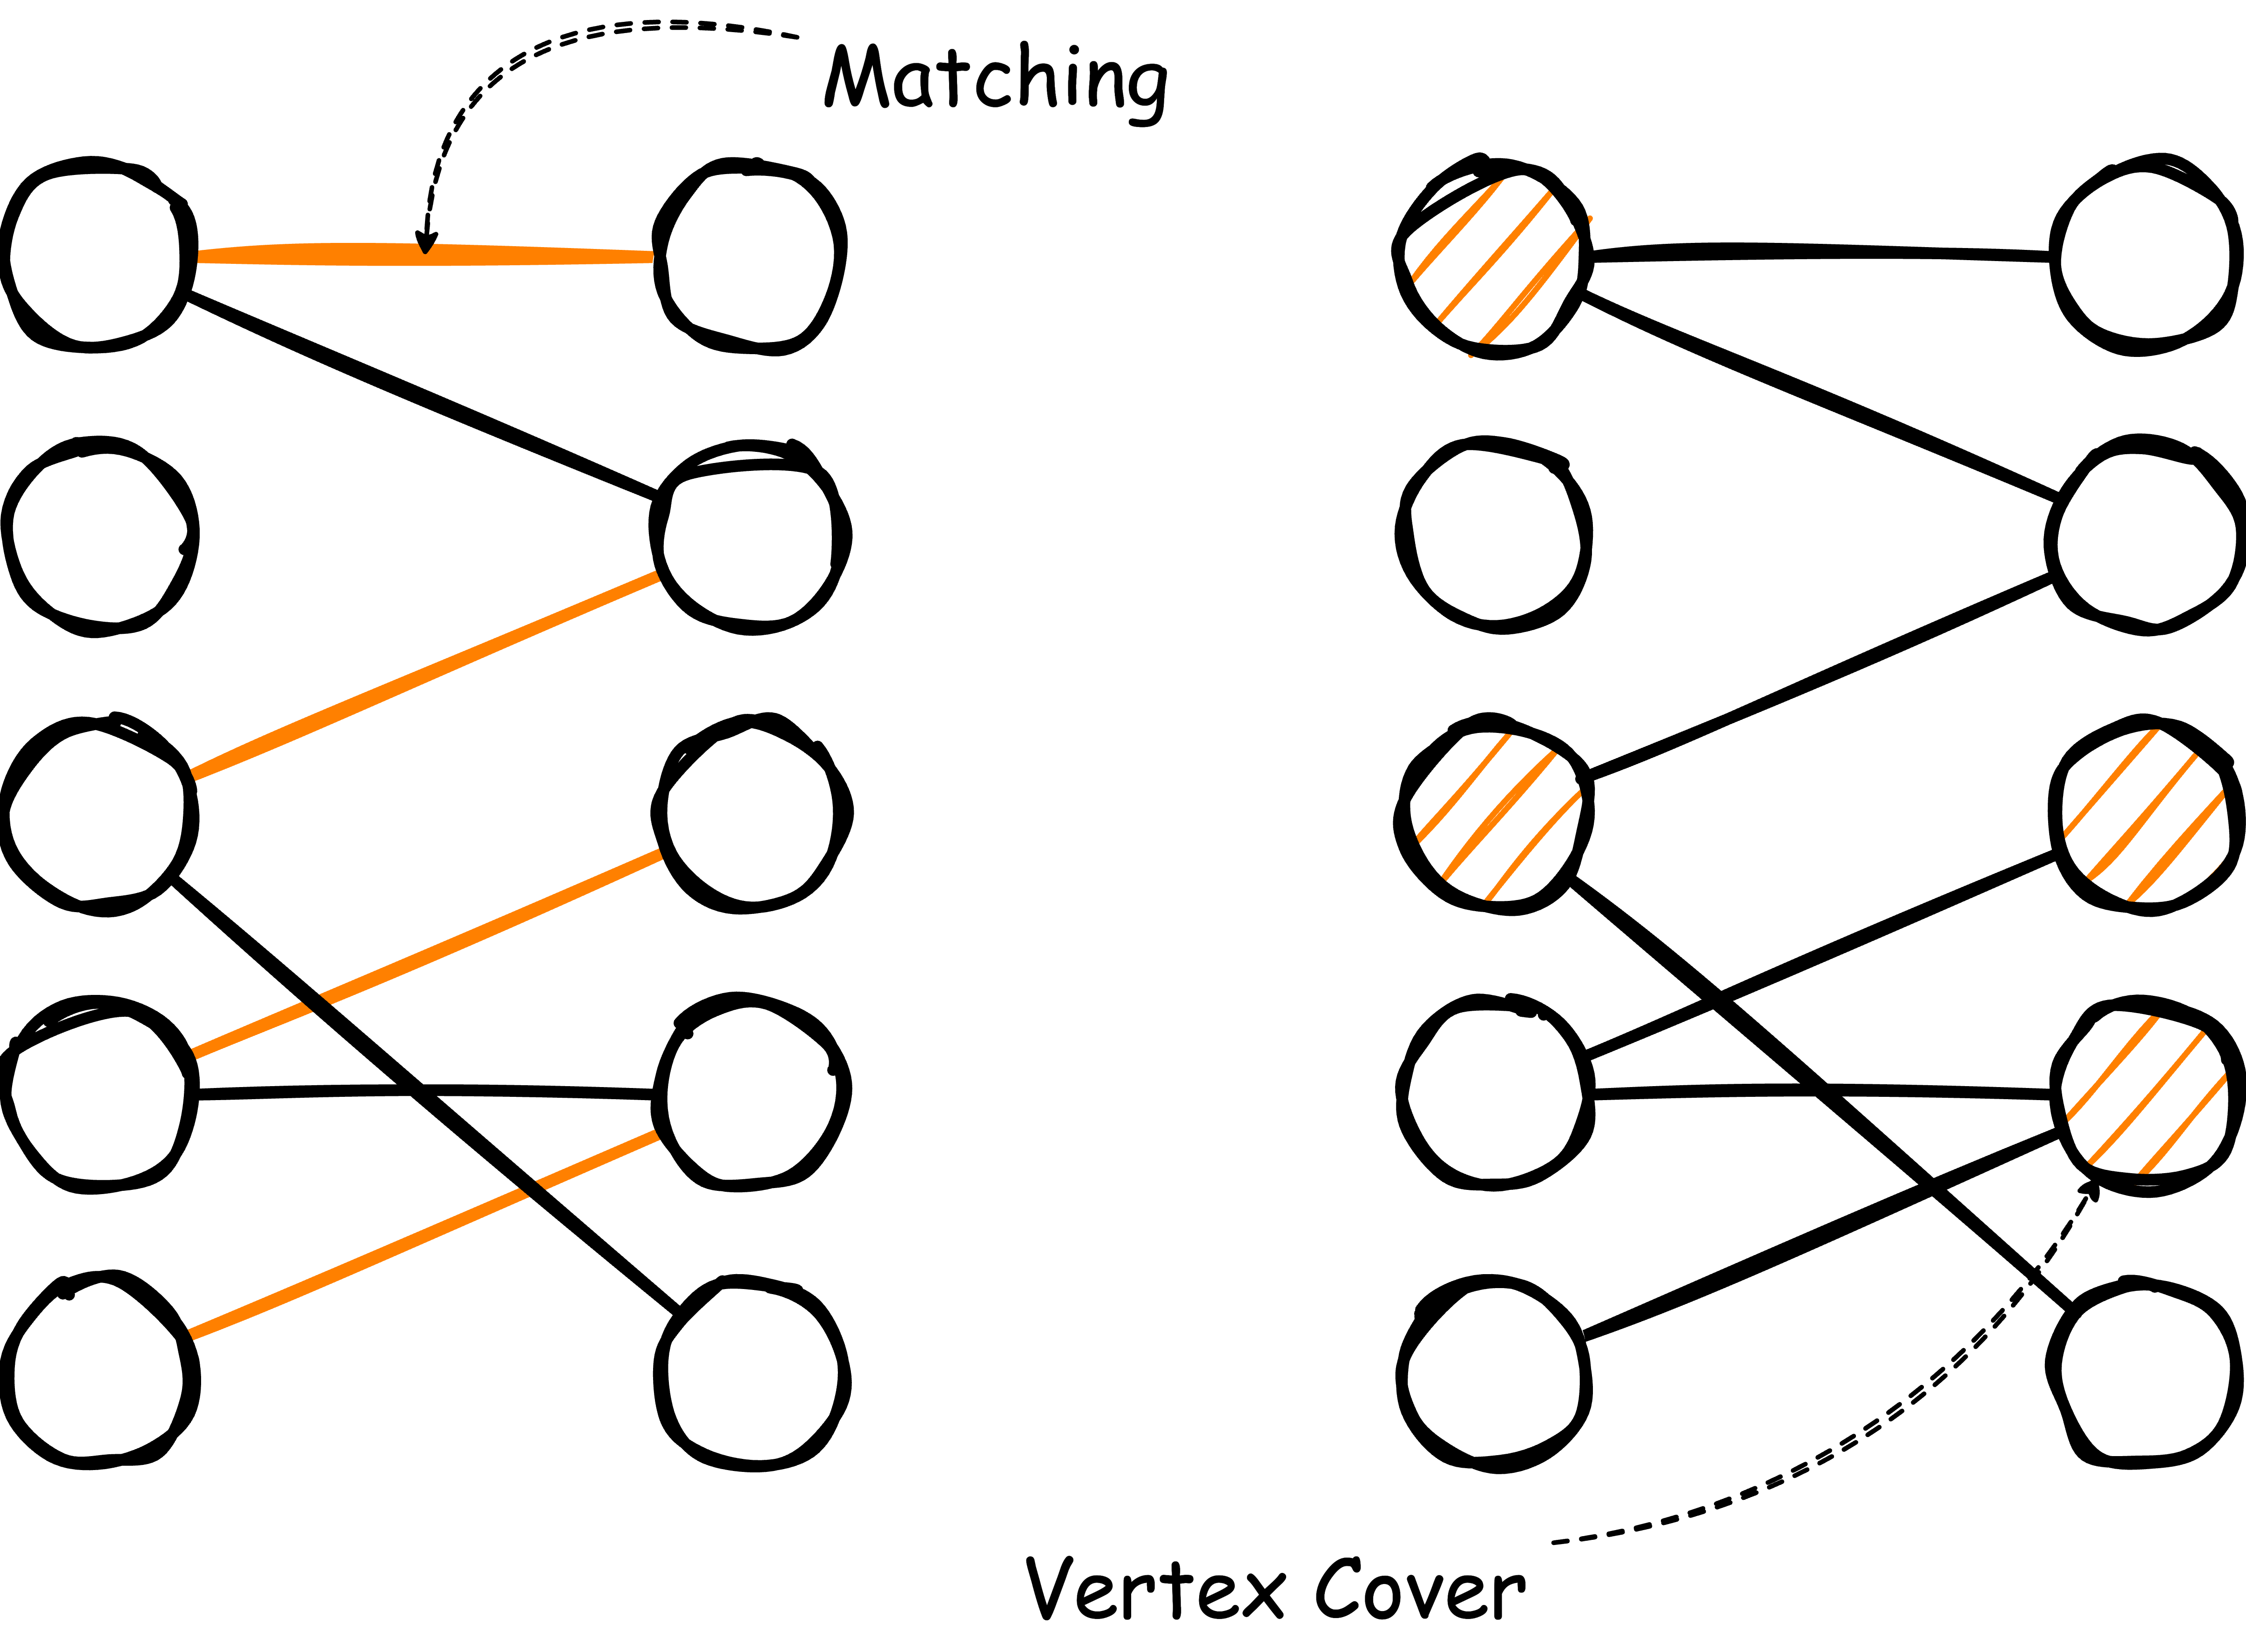
\includegraphics[width=0.9\textwidth]{figures/konigs-theorem.drawio.png}
				\end{figure}
			\end{column}
			\begin{column}{0.5\textwidth}
				\begin{figure}
					\centering
					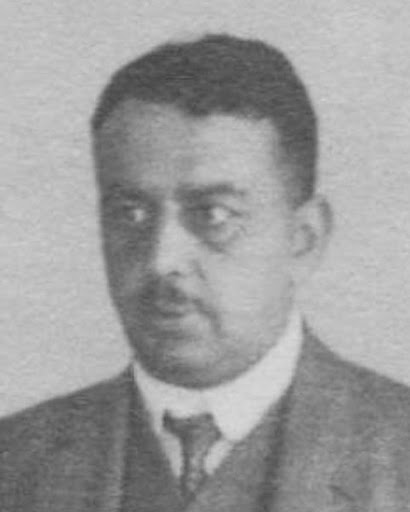
\includegraphics[width=0.5\textwidth]{figures/denes-konig.jpg}
					\caption{Dénes Konig (1884-1944)}
				\end{figure}
			\end{column}
		\end{columns}
	}

	\only<2>{
		\structure{Sketch of the proof.}

		\begin{itemize}
			\item 二部グラフ \(G\) から有向グラフ \(G'\) を構築する
			\item 最大フロー最小カット定理と下記の事実を利用する
			      \begin{itemize}
				      \item \(G'\) の\alert{最大フロー}の値 = \(G\) の\alert{最大マッチング}のサイズ
				      \item \(G'\) の\alert{最小カット}の容量 = \(G\) の\alert{最小点カバー}のサイズ
			      \end{itemize}
		\end{itemize}

		\vskip 1em

		\begin{theorem*}[最大フロー最小カット定理]
			任意の有向グラフにおいて，始点と終点が与えられたとき，\alert{最大フロー}の値は\alert{最小カット}の容量に等しい．
		\end{theorem*}
	}
\end{frame}

\begin{frame}{二部グラフ \(G\) からの有向グラフ \(G'\) を構成する方法}
	\(G = (U \sqcup V, E)\) を二部グラフとする．有向グラフ \(G'\) を下記のように構成する．
	\small{
		\begin{itemize}
			\item 頂点集合: \(V(G') = U \cup V \cup \{s, t\}\)
			\item 辺集合: \(E(G') = \{(s, u) \mid u \in U\} \cup \{(u, v) \mid {u, v} \in E \land u \in U, v \in V\} \cup \{(v, t) \mid v \in V\}\)
		\end{itemize}
	}

	\begin{figure}
		\centering
		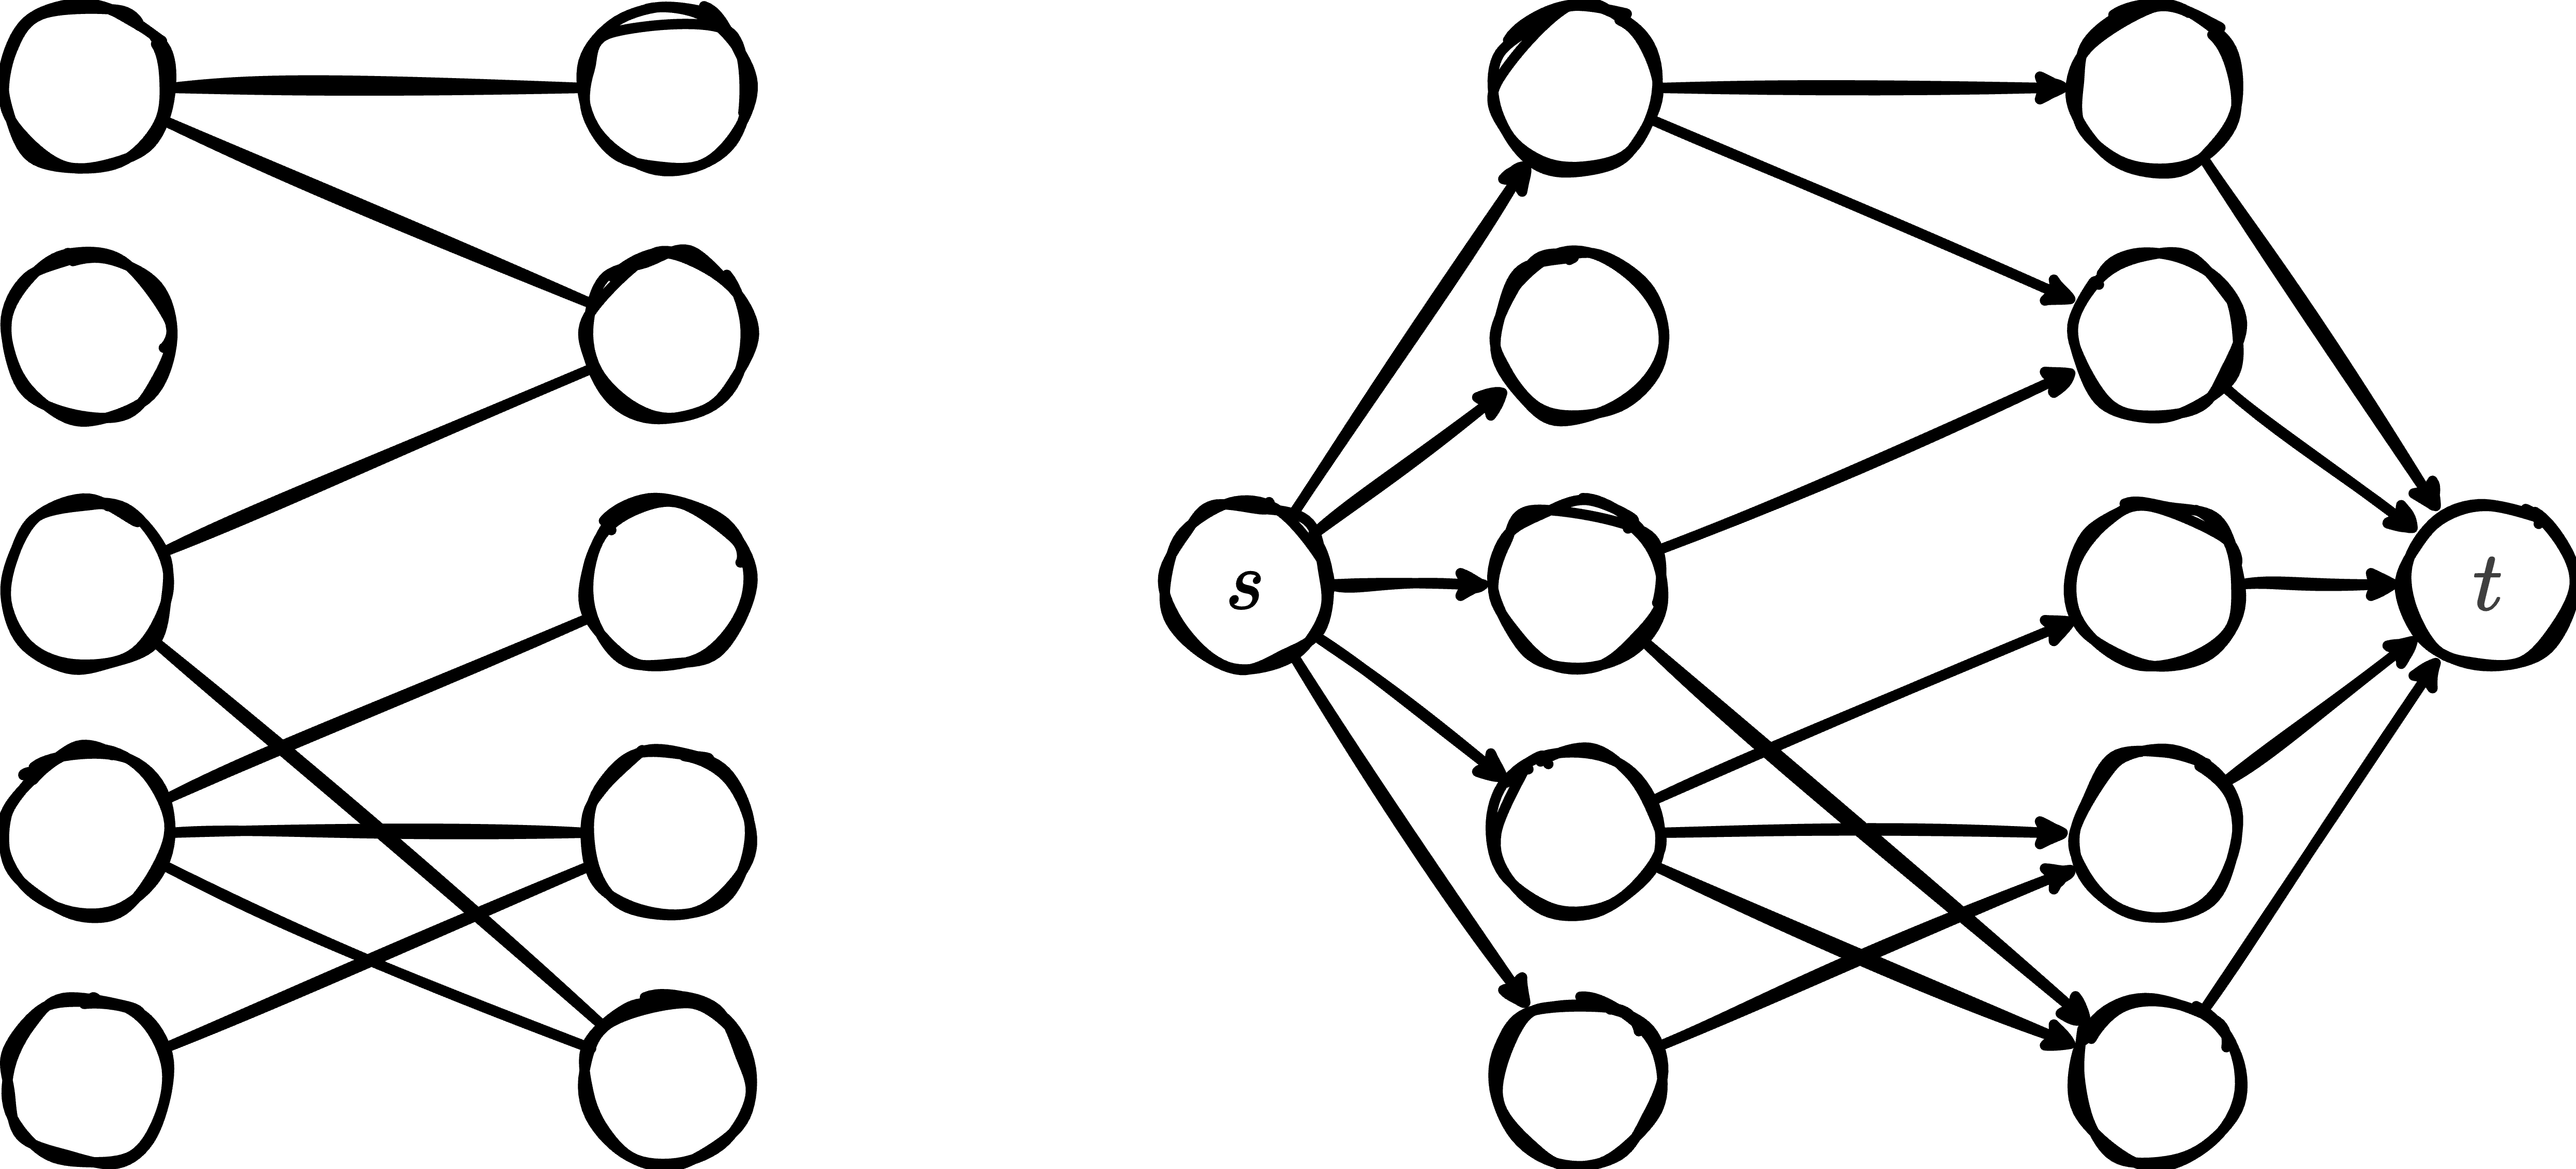
\includegraphics[width=0.75\textwidth]{figures/konig-theorem/bipartite-to-directed.png}
	\end{figure}
\end{frame}

\begin{frame}{最大フローと最大マッチングの関係}
	\(G\) での任意のマッチングは，同じ流量を持つ \(G'\) でのフローに一意に対応する．

	\begin{figure}
		\centering
		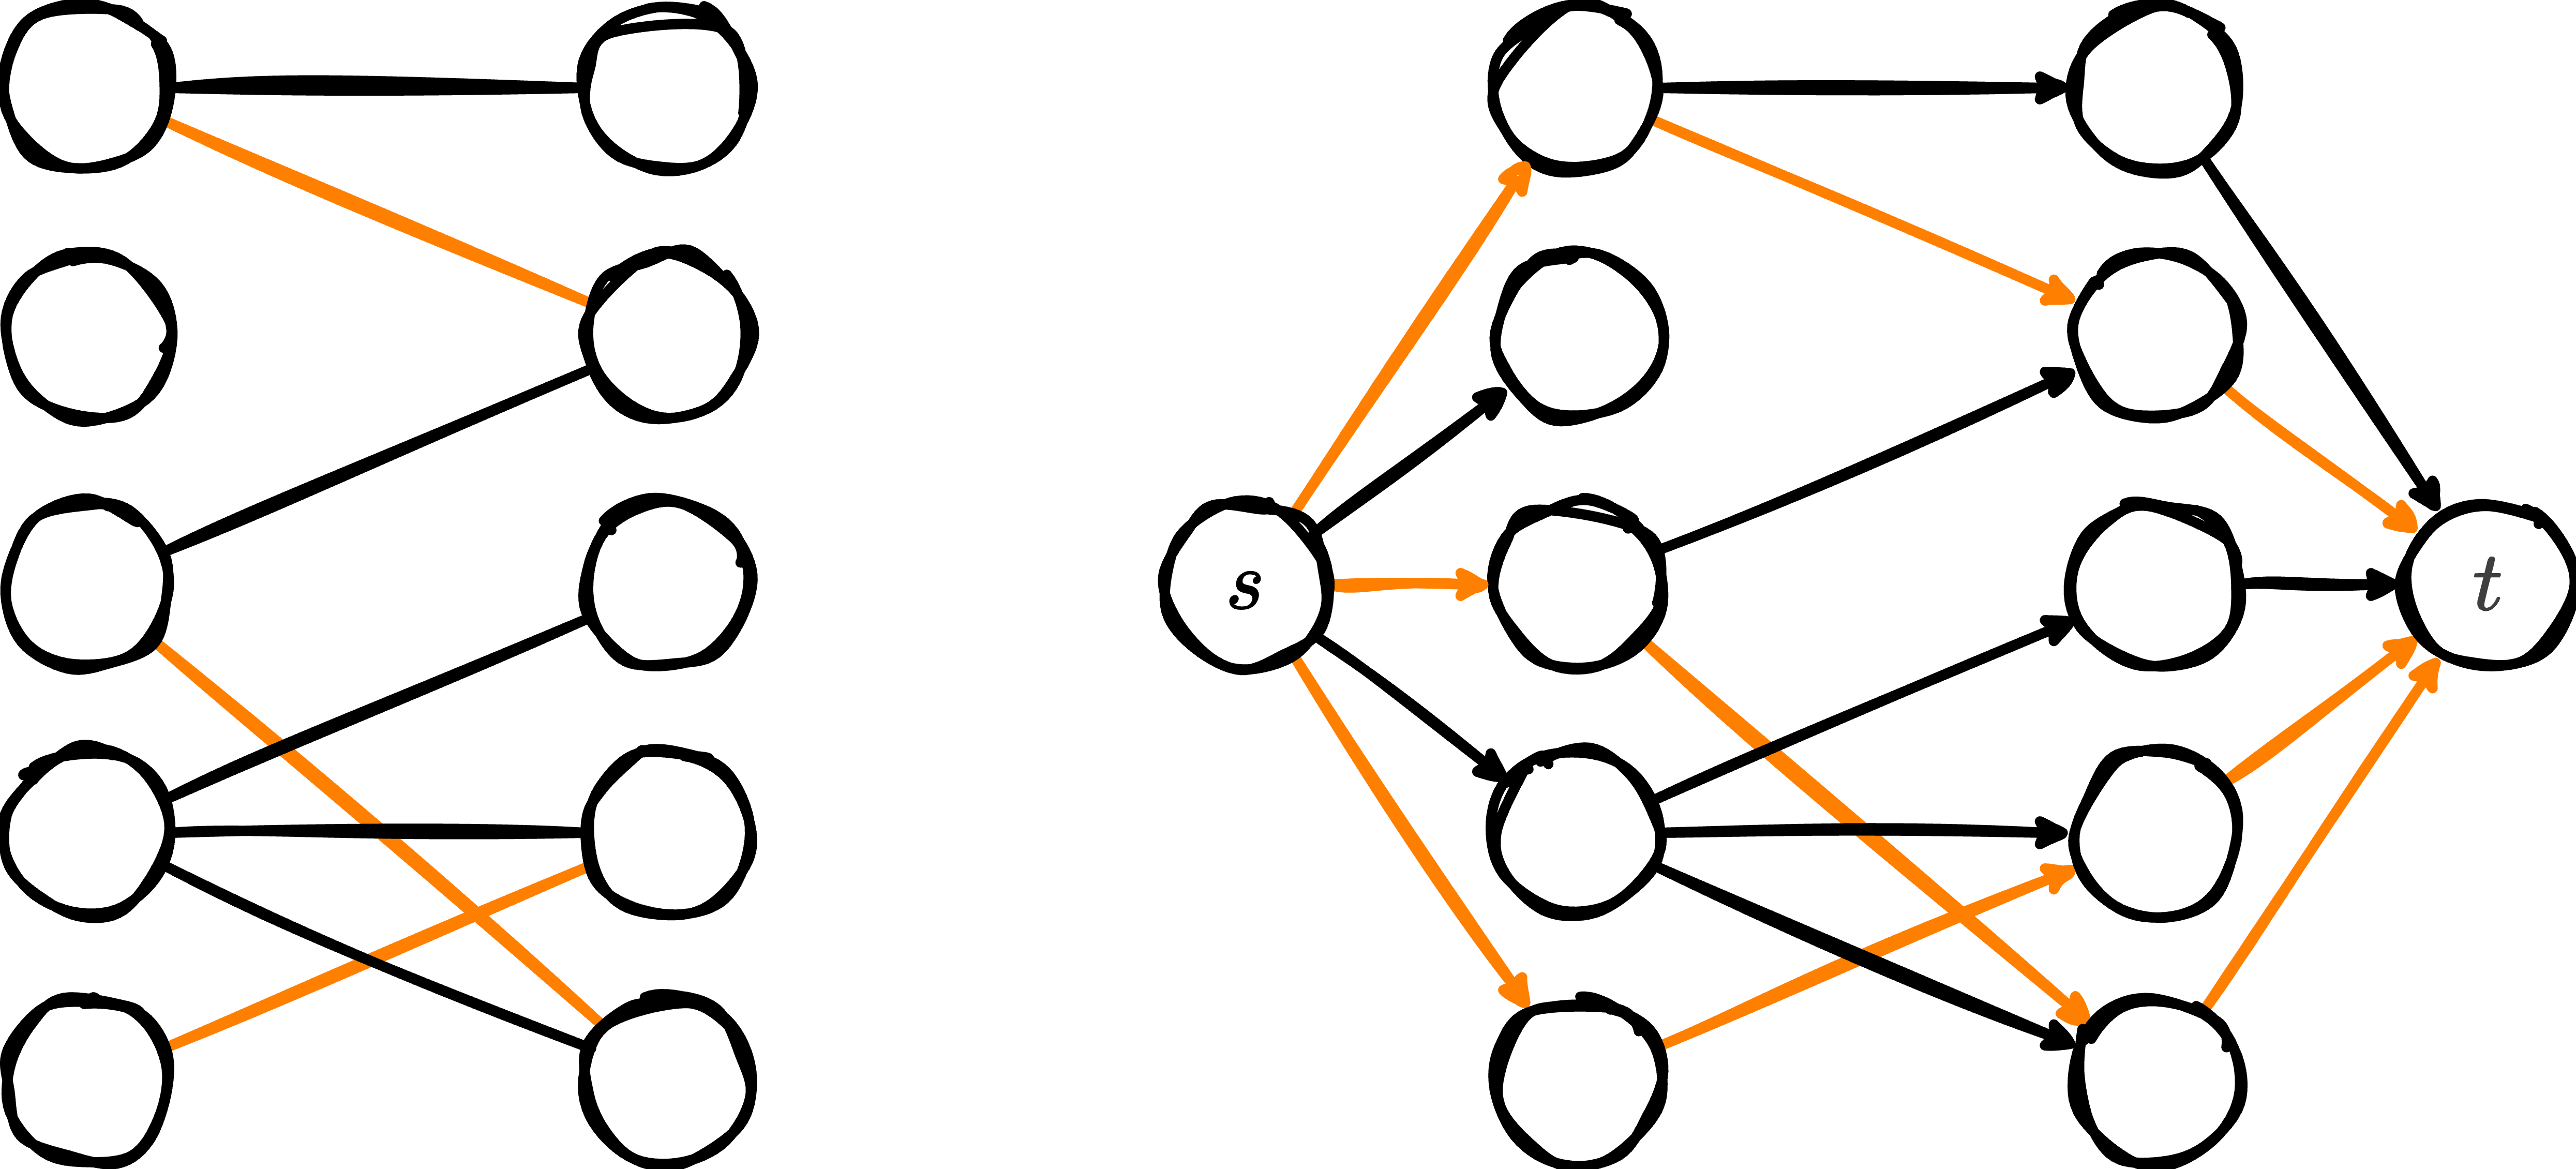
\includegraphics[width=0.75\textwidth]{figures/konig-theorem/max-flow-max-matching.png}
	\end{figure}

	\centering{\alert{\(G\) の最大マッチングのサイズ = \(G'\) の最大フローの値}}
\end{frame}

\begin{frame}{最小カットの最小点カバーの関係：\(G\) の最小点カバー \(\ge\) \(G'\) の最小カット}
	\only<1>{
		\begin{block}{示すこと}
			\(G\) の任意の点カバー \(X\) に対して，\(G'\) のカット \((S, V(G') \setminus S)\) が存在して，その容量が \(|X|\) 以下である．
		\end{block}

		\(G\) の任意の点カバー \(X\) を考える．
		\begin{figure}
			\centering
			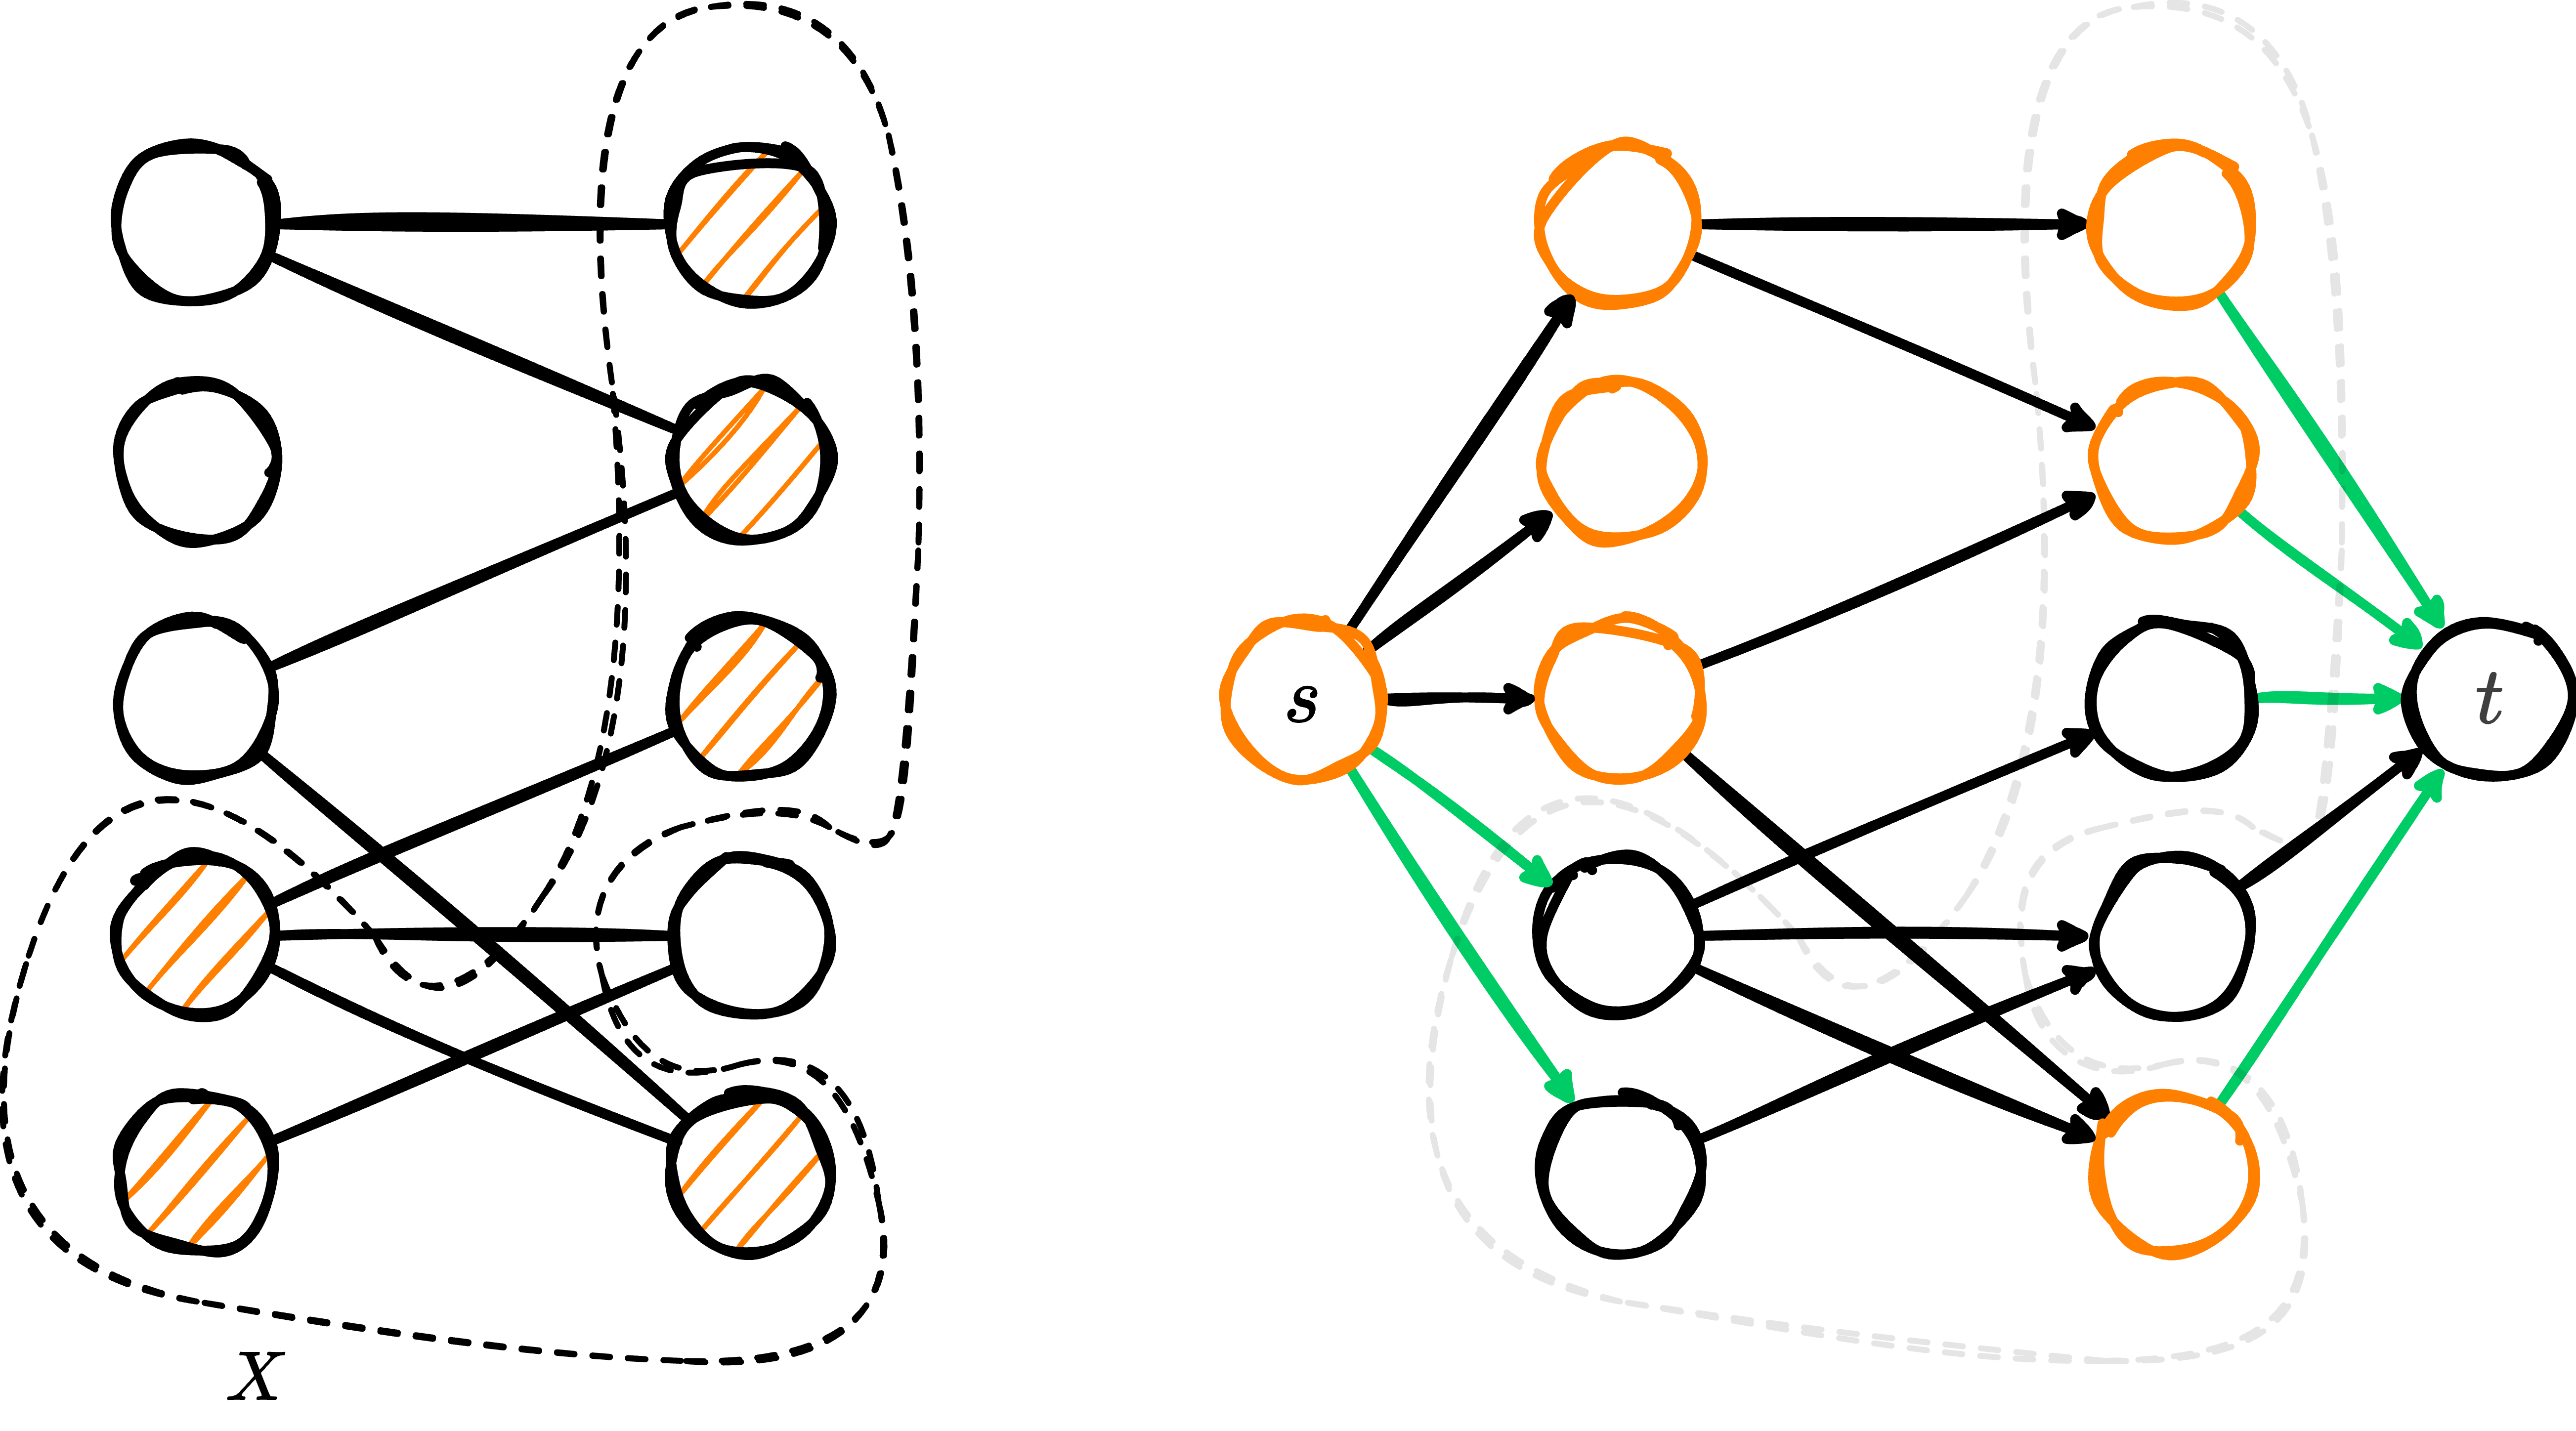
\includegraphics[width=0.6\textwidth]{figures/konig-theorem/01.png}
		\end{figure}
	}

	\only<2>{
		\begin{columns}
			\begin{column}{0.4\textwidth}
				\begin{figure}
					\centering
					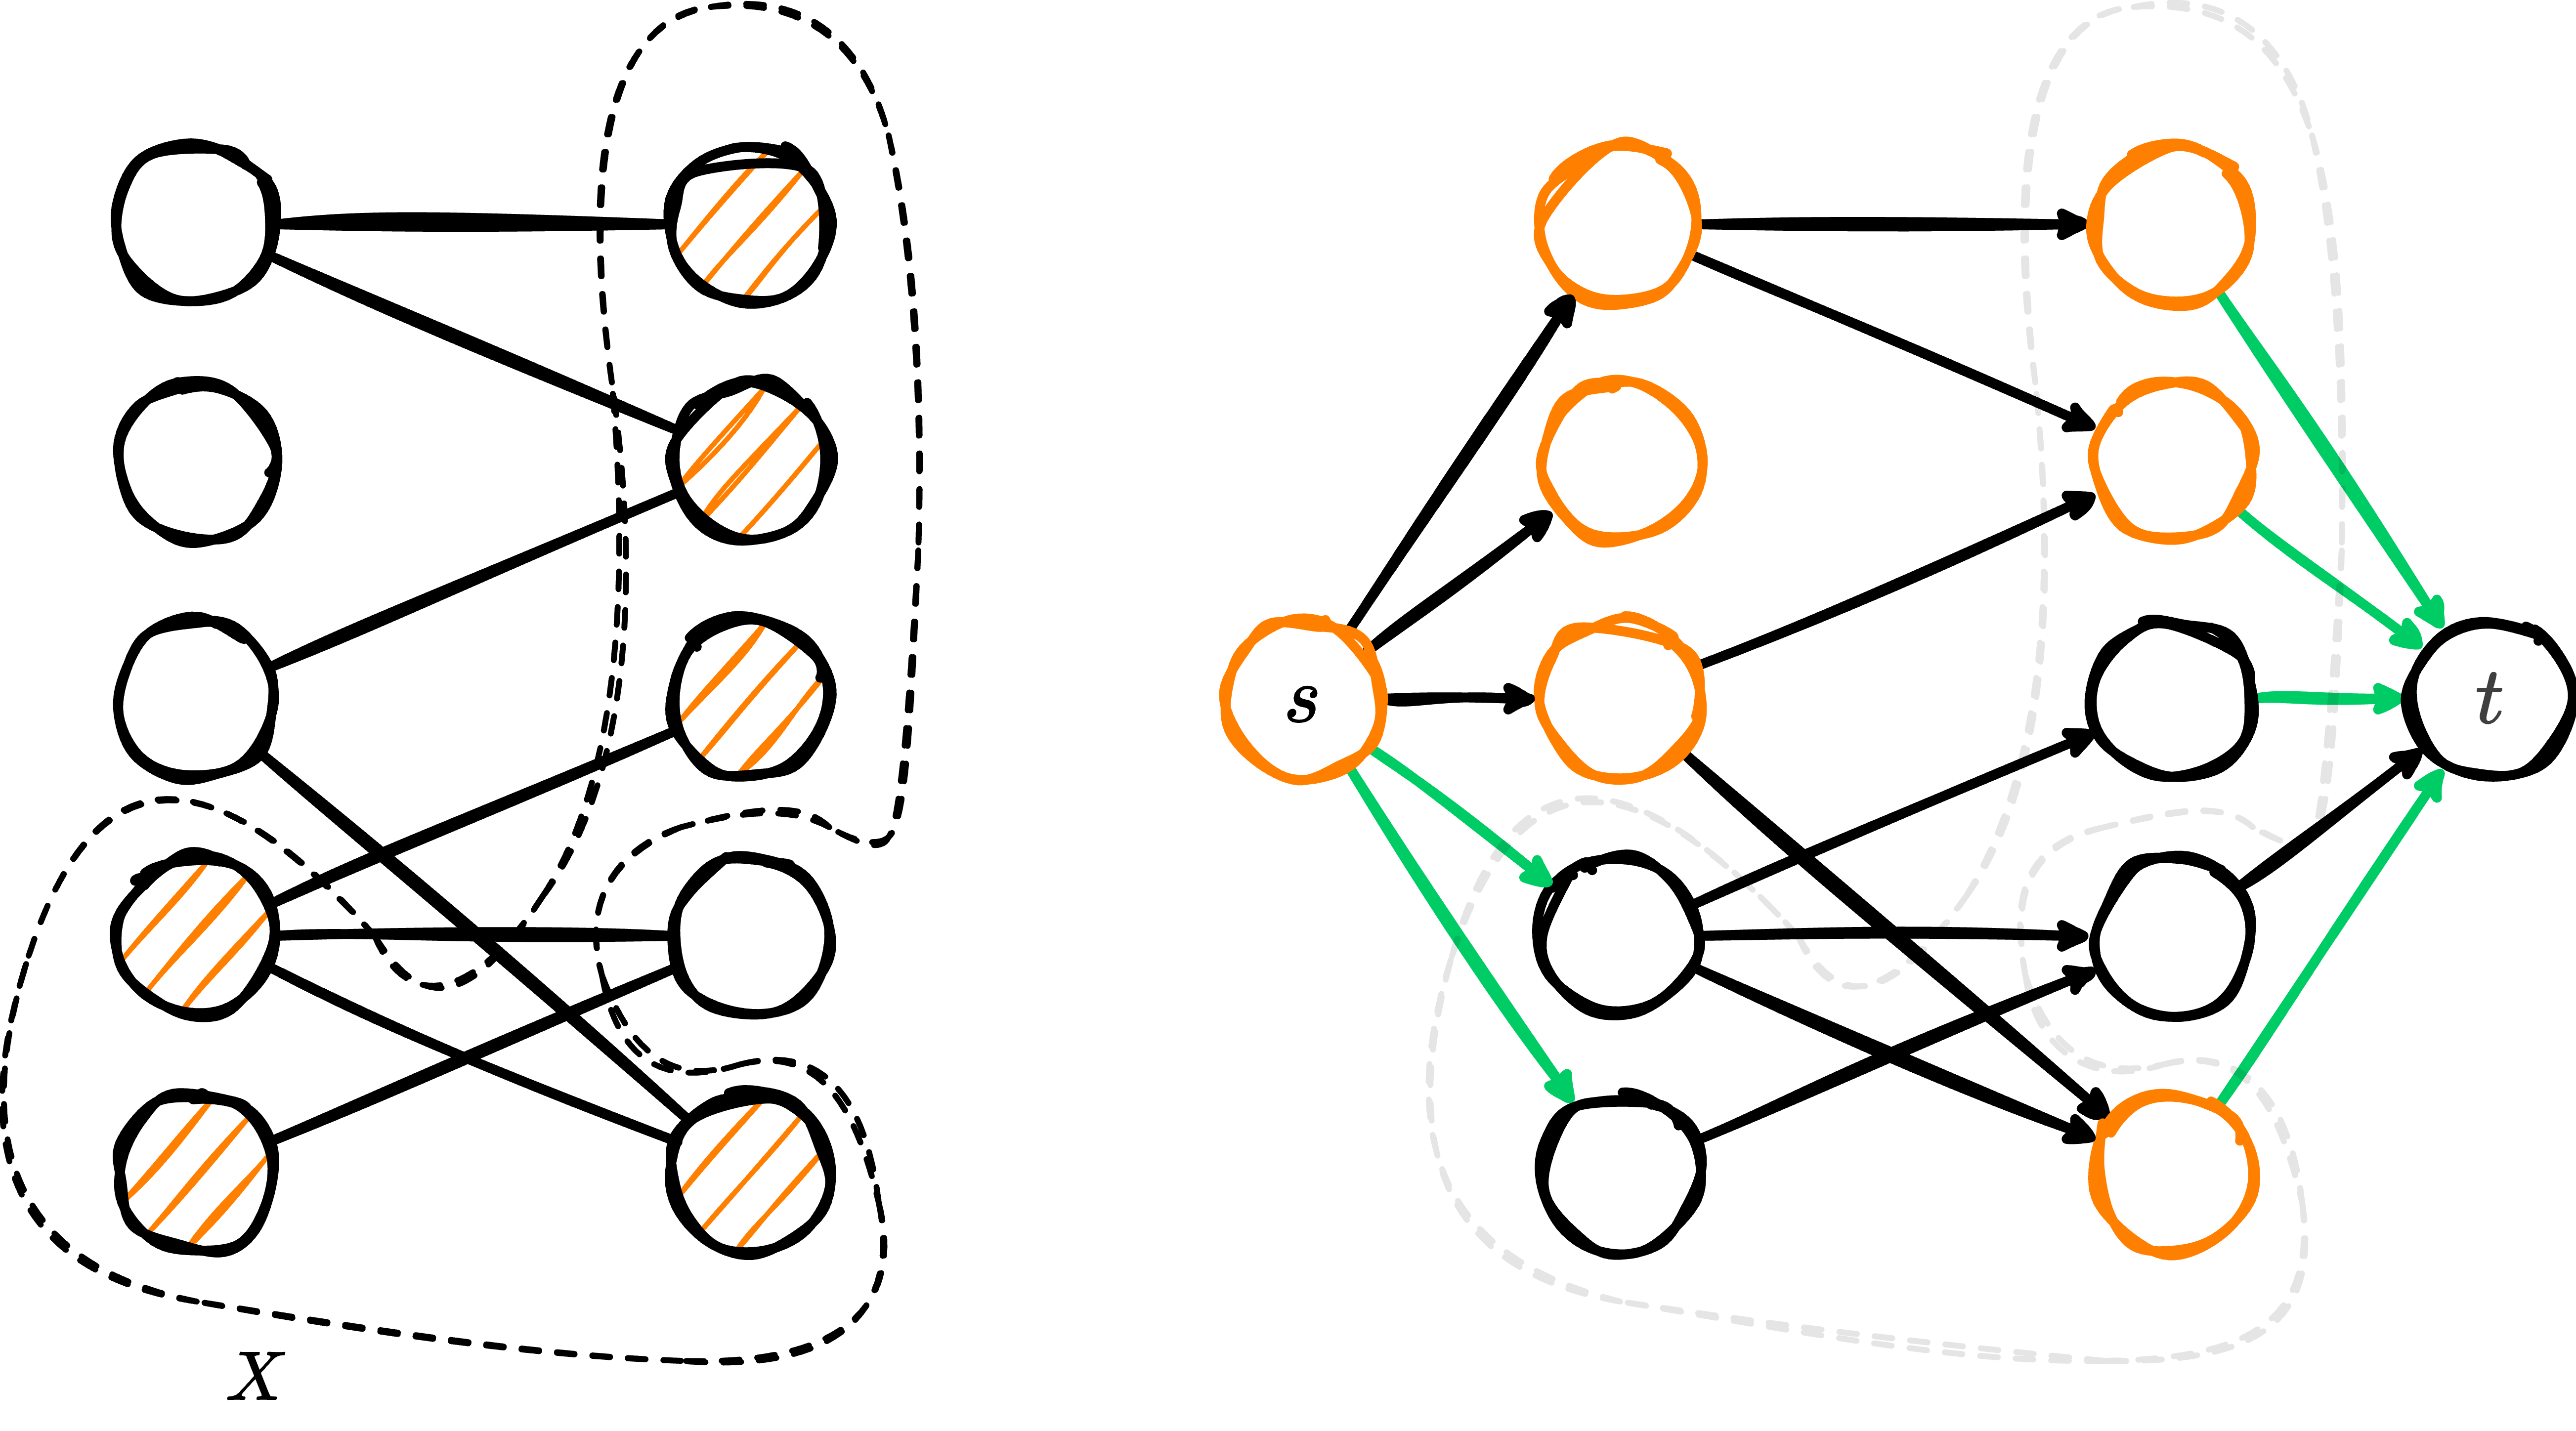
\includegraphics[width=1.0\textwidth]{figures/konig-theorem/01.png}
				\end{figure}
			\end{column}
			\begin{column}{0.6\textwidth}
				\begin{itemize}
					\item \(\info{E_X} = \{(s, u) \mid u \in U \land u \in X\} \cup \{(v, t) \mid v \in V \land v \in X\}\) と定める
					\item \alert{\(S\)} を \info{\(E_X\)} の辺を \(G'\) から削除したときの \(s\) を含む連結成分と定める
					\item[] \(\quad\quad\quad\quad\quad\quad\quad\quad \Downarrow\)
					\item \((\alert{S}, V \setminus S)\) は \(G'\) の \(s-t\) カットであることがわかる\footnote{もし \(t \in V \setminus S\) であれば，\(X\) は点カバーではないことに注意する．}
					\item \((\alert{S}, V\setminus S)\) の容量は \(|\info{E_X}| = |X|\) 以下である\footnote{\(\alert{S}\) から \(V \setminus S\) への辺が全て \info{\(E_X\)} に含まれることに注意する．}
				\end{itemize}
			\end{column}
		\end{columns}
	}
\end{frame}


\begin{frame}{最小カットの最小点カバーの関係：\(G\) の最小点カバー \(\le\) \(G'\) の最小カット}
	\only<1>{
		\begin{block}{示すこと}
			\(G'\) の任意のカット \((S, V(G') \setminus S)\) に対して，\(G\) の点カバー \(X\) が存在して，そのサイズがカットの容量以下である．
		\end{block}

		\(G'\) の任意のカット \(C = (S, V(G') \setminus S)\) を考える．
		\begin{figure}
			\centering
			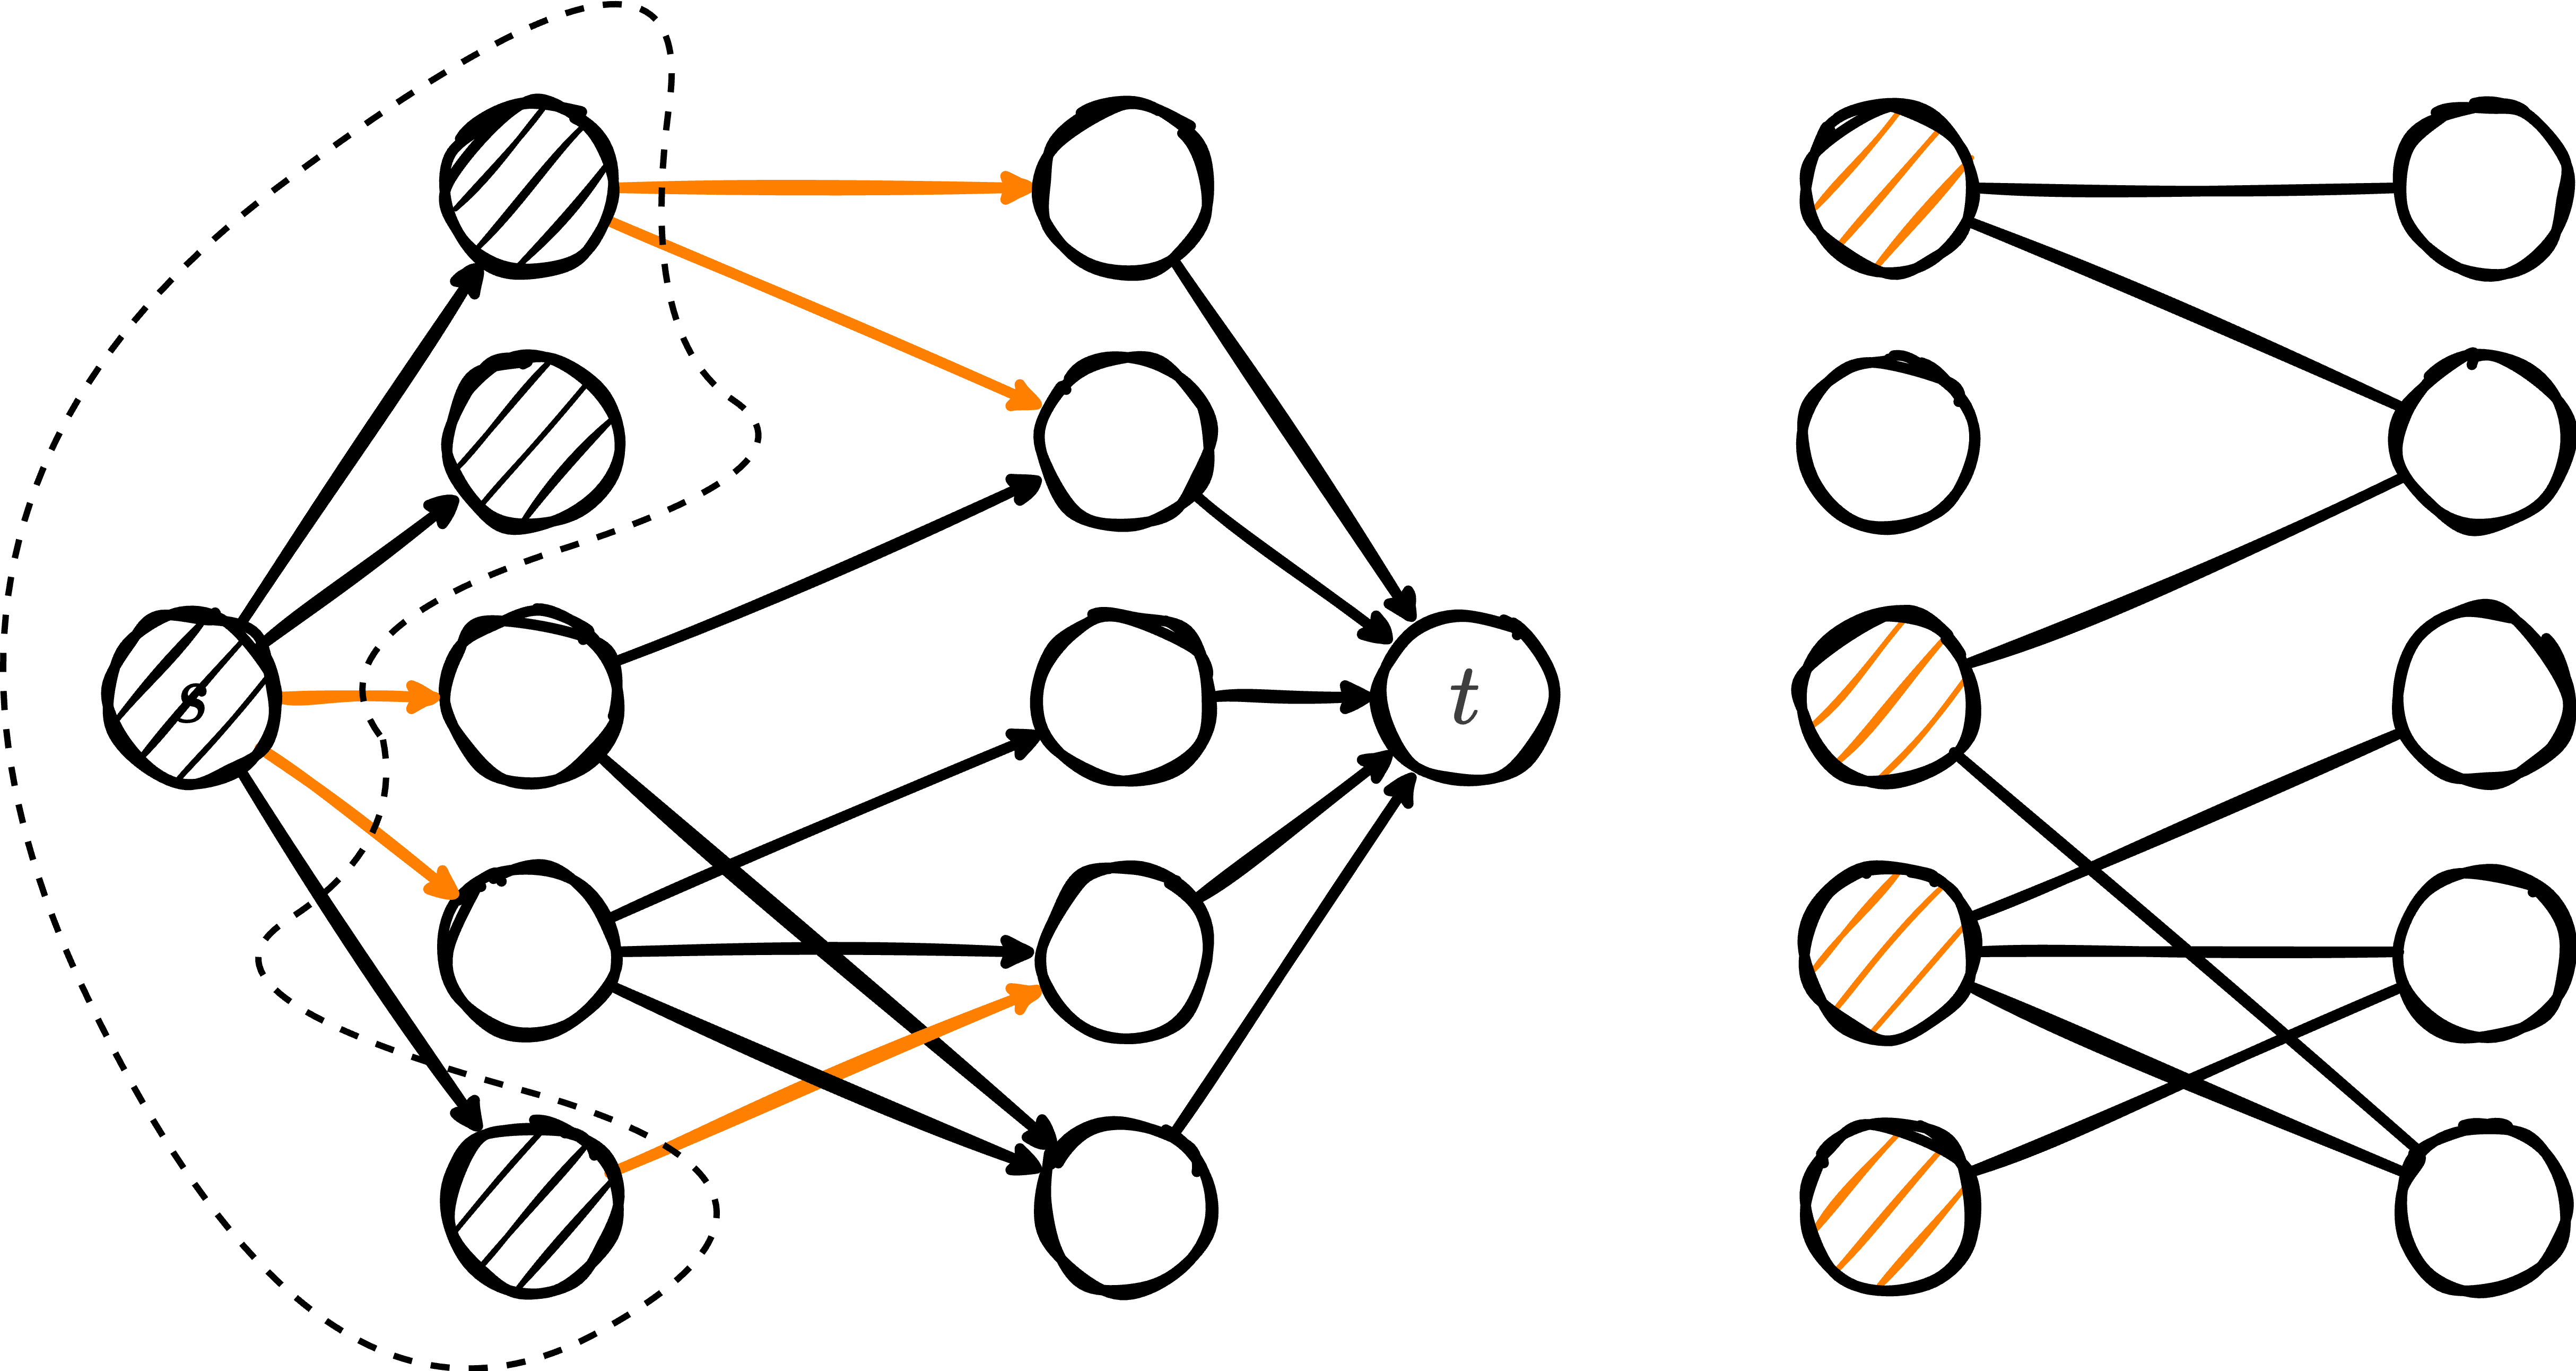
\includegraphics[width=0.6\textwidth]{figures/konig-theorem/02.png}
		\end{figure}
	}

	\only<2>{
		\begin{columns}
			\begin{column}{0.4\textwidth}
				\begin{figure}
					\centering
					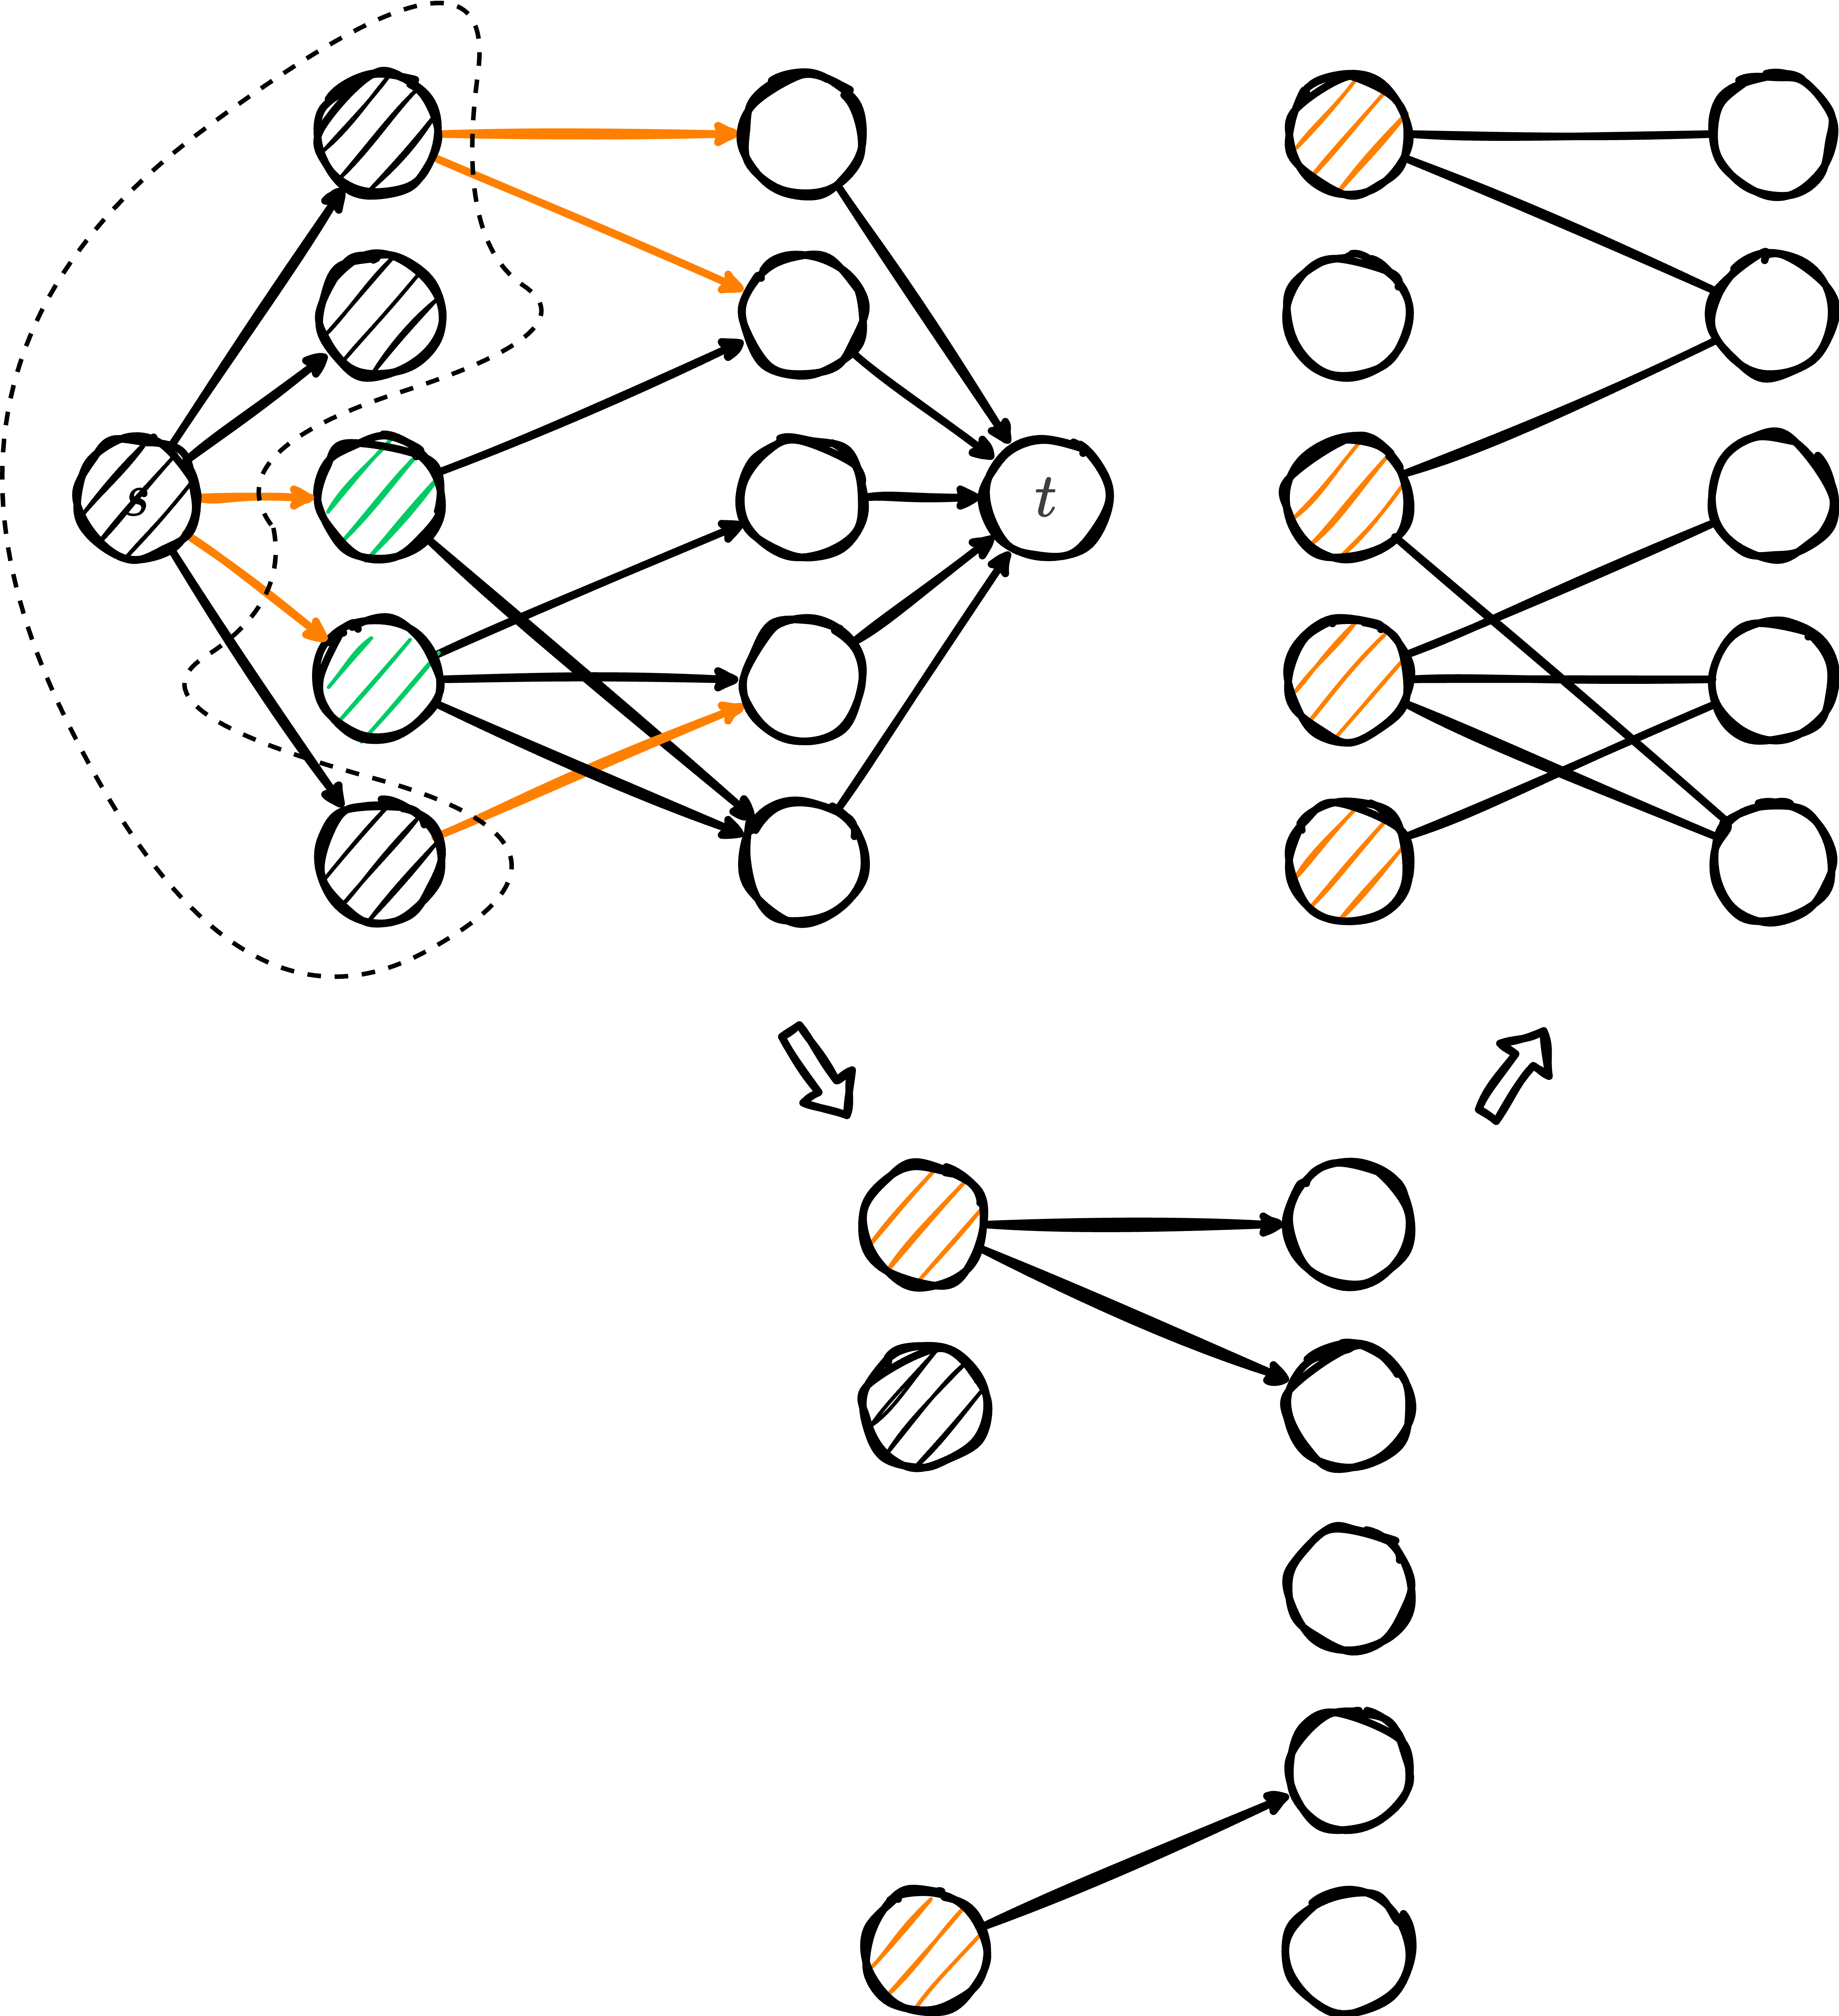
\includegraphics[width=1.0\textwidth]{figures/konig-theorem/03.png}
				\end{figure}
			\end{column}
			\begin{column}{0.6\textwidth}
				\begin{itemize}
					\item \(\info{X} = \{u \in U \mid u \in S\} \cup \{v \in V \mid v \notin S\}\) と定める
					\item \(\alert{X'}\) を \(X\) と \(G[(U \sqcup V) \setminus \info{X}]\) において出次数 1 以上の頂点との和集合と定める
					\item[] \(\quad\quad\quad\quad\quad\quad\quad\quad \Downarrow\)
					\item \(\alert{X'}\) は \(G\) の点カバーであることがわかる
					\item \(C\) の容量は \(|\alert{X'}|\) 以下である
					      \begin{itemize}
						      \item \(|\info{X}|\) は \(C\) の左右の辺の数以下である
						      \item \(|\alert{X'}|\) と \(|\info{X}|\) の差分は \(G[(U \sqcup V) \setminus \info{X}]\) の辺の数以下である
						      \item \(G[(U \sqcup V) \setminus \info{X}]\) の辺に対応する \(G'\) の辺は全て \(C\) に含まれる
					      \end{itemize}
				\end{itemize}
			\end{column}
		\end{columns}
	}
\end{frame}

\begin{frame}{最小カットと最小点カバーの関係}
	\begin{block}{示したこと}
		\(G\) の任意の点カバー \(X\) に対して，\(G'\) のカット \((S, V(G') \setminus S)\) が存在して，その容量が \(|X|\) 以下である．
	\end{block}
	\begin{block}{示したこと}
		\(G'\) の任意のカット \((S, V(G') \setminus S)\) に対して，\(G\) の点カバー \(X\) が存在して，そのサイズがカットの容量以下である．
	\end{block}
	\centering{\alert{\(G\) の最小点カバーの点数 = \(G'\) の最小カットの容量}}
\end{frame}

\begin{frame}[allowframebreaks]{References}
	\printbibliography{}
\end{frame}

\begin{frame}{Special Thanks}
	\begin{itemize}
		\item ある行列が完全単模行列であることの証明: \url{http://dopal.cs.uec.ac.jp/okamotoy/lect/2014/fdopt/handout07.pdf}
		\item 線形計画法の基本定理の証明: \url{https://ja.wikipedia.org/w/index.php?title=線形計画法の基本定理}
	\end{itemize}
\end{frame}

\begin{frame}[standout]
	Any Questions?
\end{frame}

\appendix

\begin{frame}{線形代数の復習 -- 集合}
	\begin{definition}[凸集合]
		集合 \(S \subseteq \mathbb{R}^n\) が\alert{凸集合}であるとは，任意の \(\boldsymbol{x}, \boldsymbol{y} \in S\) と \(0 \leq \lambda \leq 1\) に対して，\(\lambda \boldsymbol{x} + (1 - \lambda) \boldsymbol{y} \in S\) が成立することをいう．
	\end{definition}

	\begin{definition}[凸多面体]
		集合 \(P \subseteq \mathbb{R}^n\) が\alert{凸多面体}であるとは，有限個の線形不等式で表される凸集合であることをいう．
	\end{definition}

	\begin{definition}[頂点]
		凸多面体 \(P\) の点 \(\boldsymbol{v} \in P\) が \(P\) の\alert{頂点}であるとは，ある \(0 < \lambda < 1\) と \(P\) の互いに異なる 2 点 \(\boldsymbol{x}, \boldsymbol{y} \in P\) に対して，\(\boldsymbol{v} = \lambda \boldsymbol{x} + (1 - \lambda) \boldsymbol{y}\) と表せないことをいう．
	\end{definition}
\end{frame}

\begin{frame}{線形代数の復習 -- 行列式とその性質}
	\begin{definition}[行列式]
		\(n \times n\) 行列 \(A = (a_{ij})\) の\alert{行列式}とは，以下の式で定義される．
		\[
			\det(A) = \sum_{\sigma \in S_n} \left( \sgn(\sigma) \prod_{i=1}^{n} a_{i, \sigma(i)} \right)
		\]
		ただし，\(S_n\) は \(n\) 次対称群，\(\sgn(\sigma)\) は置換 \(\sigma\) の符号を表す．
	\end{definition}

	\begin{itemize}
		\item \(A\) の \(i\) 行と \(j\) 行を入れ替えると，\(\det(A)\) は符号が変わる
		\item \(A\) の \(i\) 行に定数倍をすると，\(\det(A)\) も同じ定数倍される
		\item \(A\) の \(i\) 行に他の行の定数倍を加えても，\(\det(A)\) は変わらない
		\item \(A\) が単位行列ならば，\(\det(A) = 1\)
		\item \(A\) が正則ならば，\(A^{-1} = \frac{\mathrm{adj}(A)}{\det(A)}\)
		      ただし，\(\mathrm{adj}(A)\) は \(A\) の随伴行列である．
	\end{itemize}
\end{frame}

\begin{frame}{線形代数の復習 -- 余因子展開}
	\begin{definition}[余因子]
		\(n \times n\) 行列 \(A = (a_{ij})\) の\alert{\(a_{ij}\) の余因子}とは，\((-1)^{i+j} \det(M_{ij})\) で定義される．
		ただし，\(M_{ij}\) は \(A\) から \(i\) 行と \(j\) 列を削除して得られる \((n-1) \times (n-1)\) 行列である．
	\end{definition}

	\begin{theorem}[余因子展開]
		\(n \times n\) 行列 \(A = (a_{ij})\) に対して，任意の \(1 \leq i \leq n\) に対して，以下の式が成立する．
		\[
			\det(A) = \sum_{j=1}^{n} a_{ij} (-1)^{i+j} \det(M_{ij})
		\]
		また，任意の \(1 \leq j \leq n\) に対して，以下の式が成立する．
		\[
			\det(A) = \sum_{i=1}^{n} a_{ij} (-1)^{i+j} \det(M_{ij})
		\]
	\end{theorem}
\end{frame}

\begin{frame}{Theorem \ref{thm:fundamental-theorem-of-linear-programming} のイメージの補強のために}
	\begin{theorem*}[線形計画法の基本定理~\cite{bertsekas1995nonlinear}]
		\(P\) を \(\mathbb{R}^n\) 上の凸多面体とし，1 つ以上の頂点を持つと仮定する．
		このとき，ある線形関数が \(P\) 上で\alert{最小値}を取るならば，その値は \(P\) の\alert{頂点}のうちの 1 つで達成される．
	\end{theorem*}

	定理の条件に合わないために，結論が成り立たない例を示す．

\end{frame}

\begin{frame}{Tools}
	\begin{theorem}[LP-双対定理]
		主問題が有界な最適解をもつための必要十分条件は双対問題が有界な最適解をもつことである．
		さらに，\(\boldsymbol{x}^*\) と \(\boldsymbol{y}^*\) がそれぞれ主問題と双対問題の最適解ならば，以下の等式が成立する．

		\[
			\boldsymbol{c}^{\top}\boldsymbol{x}^* = \boldsymbol{b}^{\top}\boldsymbol{y}^*
		\]

	\end{theorem}

	\begin{theorem}[弱双対定理]
		\(\boldsymbol{x}\) と \(\boldsymbol{y}\) がそれぞれ主問題と双対問題の実行可能解ならば，以下の不等式が成立する．
		\[
			\boldsymbol{c}^{\top}\boldsymbol{x} \leq \boldsymbol{b}^{\top}\boldsymbol{y}
		\]
	\end{theorem}

\end{frame}

\begin{frame}{Tools 2}
	\begin{theorem}[相補条件]
		\(\boldsymbol{x}\) と \(\boldsymbol{y}\) をそれぞれ主問題と双対問題の実行可能解とする．
		このとき，\(\boldsymbol{x}\) と \(\boldsymbol{y}\) がそれぞれ最適解であるための必要十分条件は，以下の条件が成立することである．

		\textbf{主相補条件: } 各 \(1 \leq j \leq n\) に対して，\(x_j = 0\) あるいは \(\sum_{i=1}^{m} a_{ij} y_i = c_j\) である．

		\textbf{双対相補条件: } 各 \(1 \leq i \leq m\) に対して，\(y_i = 0\) あるいは \(\sum_{j=1}^{n} a_{ij} x_j = b_i\) である．
	\end{theorem}
\end{frame}


\end{document}
